\documentclass[10pt,twocolumn]{confpaper}

%%%%%%%%%%%%%%%%%%%%  INCLUDES  %%%%%%%%%%%%%%%%%%%%%%%%%%

\definecolor{darkgreen}{rgb}{0.0, 0.65, 0.0}

\ifthenelse{\equal{\COMMENTS}{yes}}{%
\newcommand{\mcnote}[1]{\textit{\textcolor{blue}{[marco]: #1}}} % Marco's comments
\newcommand{\lv}[1]{\textcolor{red}{(\textit{\textcolor{red}{LV:#1}} )}}
\newcommand{\rmnote}[1]{\textit{\textcolor{darkgreen}{[robert]: #1}}} % Robert's comments
\newcommand{\rbnote}[1]{\textit{\textcolor{orange}{[rudy]: #1}}} % Rudy's comments
\newcommand{\nf}[1]{\textcolor{red}{(\textit{\textcolor{red}{NF: #1}} )}}
}{
\newcommand{\mcnote}[1]{}
\newcommand{\lv}[1]{}
\newcommand{\rmnote}[1]{}
\newcommand{\rbnote}[1]{}
\newcommand{\nf}[1]{}
}


\newcommand{\supsym}[1]{\raisebox{4pt}{{\footnotesize #1}}}
\newcommand{\et}{\supsym{$\dag$}}
\newcommand{\ucl}{\supsym{$\diamond$}}
\newcommand{\ptn}{\supsym{$\star$}}
\newcommand{\ceq}{\supsym{$\ddag$}}


\usepackage{listing}
\usepackage[]{algorithm2e}
\usepackage{bbm}
\usepackage{amsmath}

\renewcommand{\baselinestretch}{1.005} 


\definecolor{steel_blue}{RGB}{70, 130, 180}

\lstset{
basicstyle=\footnotesize\ttfamily\small,
frame=none,
language=Python,
numbers=none,
breaklines=true,
xleftmargin=0pt
}


\lstdefinelanguage{Pyretic}
{keywords={>>, >+, +, &, push, if_, elif_, else, pop, match, fwd, modify, set, mod, drop, $\triangleleft$, announce, withdraw}, 
  sensitive=true, alsoletter={-,>>,+,&,|,_},comment=[l][\footnotesize\sffamily\textbf]{\!}
}

\lstset{emph={View1, CA, CA-IN, as-path, med, no-prepend},
  keywordstyle=\color{steel_blue}\textbf}
\lstset{language=Pyretic}


%%%%%%%%%%%%%%%%%%%%  LOCALS  %%%%%%%%%%%%%%%%%%%%%%%%%%%%

\newcommand{\system}{iSDX\xspace}

%%%%%%%%%%%%%%%%%%%%  TITLE/AUTHORS  %%%%%%%%%%%%%%%%%%%%%


\date{}
\title{
{Concise Encoding of Flow Attributes in SDN Switches}}
\author{
{Robert MacDavid\ptn, R\"udiger Birkner\et, Ori Rottenstreich\ptn,}\\
{Arpit Gupta\ptn, Jennifer Rexford\ptn, Nick Feamster\ptn}\\
\ptn\normalsize{Princeton University}~~~\et\normalsize{ETH Z\"{u}rich}\\
}

%%%%%%%%%%%%%%%%%%%%  START OF DOCUMENT  %%%%%%%%%%%%%%%%%

\begin{document}
\maketitle
\thispagestyle{empty}

%\AcmCopyright
%\ToAppear

%\begin{sloppypar}

\abstract{
Network devices such as routers, switches, and firewalls forward traffic based on entries in their local forwarding tables. Although these forwarding tables conventionally make decisions based on a packet header field such as a destination address, attaching sets of attributes to flows during classification and making forwarding decisions based on attributes in that set can enable richer network policies. For example, devices at the edge of a network could add a tag to each packet that encodes a set of middleboxes to traverse, a set of egress locations, or a set of anycast destinations; simpler devices in the core of the network could then forward packets based on this tag. 

Unfortunately, naive construction of these tags can create forwarding tables that grow quadratically with the number of elements in the set or sequence--prohibitive for commodity network devices. In this paper, we present a compression algorithm that makes such encodings practical. The compression algorithm encodes sequences or sets (e.g., middlebox service chains, lists of next-hop network devices) in a compact tag that fits in a small packet header field. Our evaluation shows that the compression technique can encode common forwarding sequences for large networks using only a few bits and that the number of forwarding rules grows linearly with the number of elements in the set or sequence.
}



\ifthenelse{\equal{\onlyAbstract}{no}}{% !onlyAbstract



\section{Introduction}
\label{sec:intro}
%%%
%%% Forwarding Equivalence Class
%%%
Routing is increasingly more sophisticated than simply directing all traffic along a shortest path to the destination.  Depending on their header fields, packets may traverse a sequence of middleboxes, be subject to access-control policies, be multicast to a set of receivers, or be anycast to one of several equivalent servers.  Customizing the handling of the packets can require network switches to have a large number of forwarding rules that match on multiple header fields.  Fortunately, many packets are treated the same way.  Traffic flows that are treated identically by the network can be grouped into a single \emph{forwarding equivalence class} (FEC). If the edge of the network classifies each packet and tags it with a FEC, the interior switches can simply forward packets based on the tag, leading to substantial reductions in forwarding state.

%%%
%%% FEC is an index
%%%
The simplest and most common form of FEC tag is a flat tag, or \emph{index}. Historically, virtual circuit switching techniques like MPLS [cite MPLS] and VLAN [cite VLAN] follow this approach, and it is common in newer works as well~\cite{flowtags, sdx}.  Using the tag as an index worked well with traditional switches that support exact matches on a single header field, such as an MPLS label, VLAN tag, or destination MAC address.  However, index tagging solutions face three scalability challenges.  First, the size of the tag limits the number of FECs (e.g., the 12-bit VLAN tag can represent at most 4096 FECs).  Second, the number of FECs traversing a switch determines the number of forwarding rules and the churn that occurs after network events like link failures. And third, index tags offer no way to easily decode attributes associated with a FEC using a small amount of switch memory. 
%If a network node wishes to decode whether attribute $A$ is associated with a packet, it must determine whether the packet belongs to any FEC which is associated with $A$. If $A$ is associated with $N$ FECs, each of which has its own index, the switch requires $N$ rules for decoding $A$. 

%%%
%%% Matching on sequences
%%%
Fundamentally, the issue is that each FEC represents a \emph{collection} of attributes, yet two FECs that differ by only one attribute receive arbitrary indices. For middlebox steering policies, the FEC represents a sequence of middleboxes, and two FECs may differ in a single hop.  If the tag could represent a list of middleboxes efficiently, then switch $B$ in the example above would need just \emph{one} rule to differentiate between packets going to $C$ and $D$.
%%%
%%% Capabilities of newer switches 
%%%
Recently, commodity switches have emerged with more sophisticated capabilities.  OpenFlow 1.3~\cite{of13} supports \emph{wildcard} matching on multiple header fields. Emerging protocol-independent switches (programmable using languages like P4~\cite{P4}) support arbitrary headers that can be read, written, and matched in flexible ways.  These advances enable much more flexible ways to tag and match packets, beyond simple index tagging. 

%In the case of virtual circuit switching, the number of possible circuits can be exponential in the size of the network. Switches need to be programmed to react to every tag they may see, resulting in exponential memory usage. It may be the case that the majority of equivalence classes that a switch sees take identical egress ports, yet traditional tagging is unable to take advantage of this redundancy. Fundamentally, an equivalence class can be characterized by a set of attributes where that set is unique to that class. If two circuits differ by only a single hop, their attribute sets are unique and they are assigned different tags. Traditional solutions make no attempt to convey the similarity of the two sets in the tags, which could allow switches to be programmed with a single rule that reacts to both tags. We refer to these solutions as \textit{flat tagging} solutions. 


%Paragraph 3: "In this paper, we show that ...". This is the key paragraph in the intro - you summarize, in one paragraph, what are the main contributions of your paper given the context you have established in paragraphs 1 and 2. What is the general approach taken? Why are the specific results significant? This paragraph must be really really good. If you can't "sell" your work at a high level in a paragraph in the intro, then you are in trouble. As a reader or reviewer, this is the paragraph that I always look for, and read very carefully.

In this paper, we show how the set of attributes that define an equivalence class can be embedded in the assigned tag. The attributes of any tag can then be individually read using a small set of wildcard rules.  Such \emph{attribute-carrying tags} are much more compact, and lead to much smaller rule tables, than index tagging solutions.  We present efficient algorithms for generating compact tags that represent either \emph{sets} or \emph{sequences} of attributes.  We show how these tags can be used in several real applications, including our SDN-based Internet exchange point~\cite{isdx}.  Additionally, we show how these tags not only improve the scalability of existing systems, but also open new applications. We have made public the code library for incorporating our tagging scheme into any application. We perform evaluations on both real and synthetic datasets for our proposed applications and show that it can reduce the amount of switch memory by X. 

%Paragraph 4: At a high level what are the differences in what you are doing, and what others have done? Keep this at a high level, you can refer to a future section where specific details and differences will be given. But it is important for the reader to know at a high level, what is new about this work compared to other work in the area.

%Paragraph 5: "The remainder of this paper is structured as follows..." Give the reader a roadmap for the rest of the paper. Avoid redundant phrasing, "In Section 2, In section 3, ... In Section 4, ... " etc.

The remainder of this paper is structured as follows. In \S \ref{sec:background}, we give some area background and a few motivating applications. In \S \ref{sec:base_encoding}, we outline the basic ideas of our encoding scheme for attaching sets of attributes to packet headers. In \S \ref{sec:identifiers}, we improve the space usage of the base encoding. In \S \ref{sec:ordering}, we extend our encoding to support ordered sequences of attributes. In \S \ref{sec:evaluation}, we evaluate the encoding over both real and synthetic data sets. We discuss related works in \S \ref{sec:related}. The paper concludes with \S \ref{sec:conclusion}.






%\subsection{Common Ground}
%
%Although a diverse set of applications, each of these problems fits a common framework. As a packet enters a local area network, it is classified as belonging to some category of traffic. Associated with this category of traffic is a sequence or set. During classification, this sequence is somehow attached to the packet header.
%All three of these examples have a common framework: Packets are fit into categories as they enter a local area network, and associated with each category is some sequence of information. These sequences can be middleboxes, hosts, next-hop switches, or something else entirely. The sequence could be ordered, as in the case of middlebox paths, or unordered as in the case of feasible next-hops. In each case, the sequence is read by the local network switches to determine which direction to route the traffic. We refer to this reading of information as \textit{membership testing}, because routing choices are decided based upon which hosts or middleboxes are members of the sequence. 

%\subsection{Forwarding Table Matching On Tags}
%
%
%For this scheme of attaching information sets to packets to be feasible with commodity switches, it must be possible for membership testing to be implemented in the forwarding tables of switches. In switch TCAM tables, rules are are comparisons between a fixed string and the packet header, where the fixed strings are over the alphabet $\{0,1,*\}$. $0$ and $1$ are specific bit values, and $*$ denotes "don't care". We say that a packet header matches a string if for every bit in the header, either the bits are equal or one is a wildcard. Example usages include exact matches (strings with no wildcards), prefix matches (strings that end in wildcards), and reading of individual bits (strings with only one non-wildcard). 
%
%Various applications benefit from the use of TCAM 
%
% (TODO: cite some tagging works like flowtags and the original SDX?) have solved the problem of associating packets with information sets by generating a tag for each unique information set and repurposing one of the fields in the header for the tag. In the FlowTags work, each middlebox path had its own set of tags, which could fit into the IP Fragment Identification field. To determine if middlebox $X$ is the next-hop, switches must compare the tag to every tag which has $X$ as a next-hop using TCAM exact matches. This can result in a TCAM entry count exponential in the number of bits in a tag. In the SDX work, each set of next-hops had a unique tag which was placed in the destination mac field. Again, to determine if next-hop $X$ is correct, the tag must be compared against every tag which contains $X$ using exact TCAM matches. 
%
%In both works, the number of bits required can be quite small, but membership tests are expensive, requiring rules exponential in the tag size. TCAM is a very limited resource, and it would be desirable to design tags with the goal of decreasing the number of entries required for membership testing. 
%
%To combat these issues, we present a compression scheme which allows
%the encoding of sequences over a large number of elements, such as service chains or lists of BGP next-hops, into a format easily queried by commodity switches. We show how, with an additional algorithm, this scheme can be used to compress both ordered and unordered sets. Finally, we evaluate our algorithms across both synthetic and real datasets, and show not only does the number of bits needed by our compression scheme compete with the number of bits needed by tags, but that that each core switch need only a constant number of entries per membership test, versus a linear number of entries for the case of flat tagging.



\section{Background}

\begin{figure}[t!] 
\begin{minipage}{1\linewidth}
\begin{subfigure}[c]{0.96\linewidth}
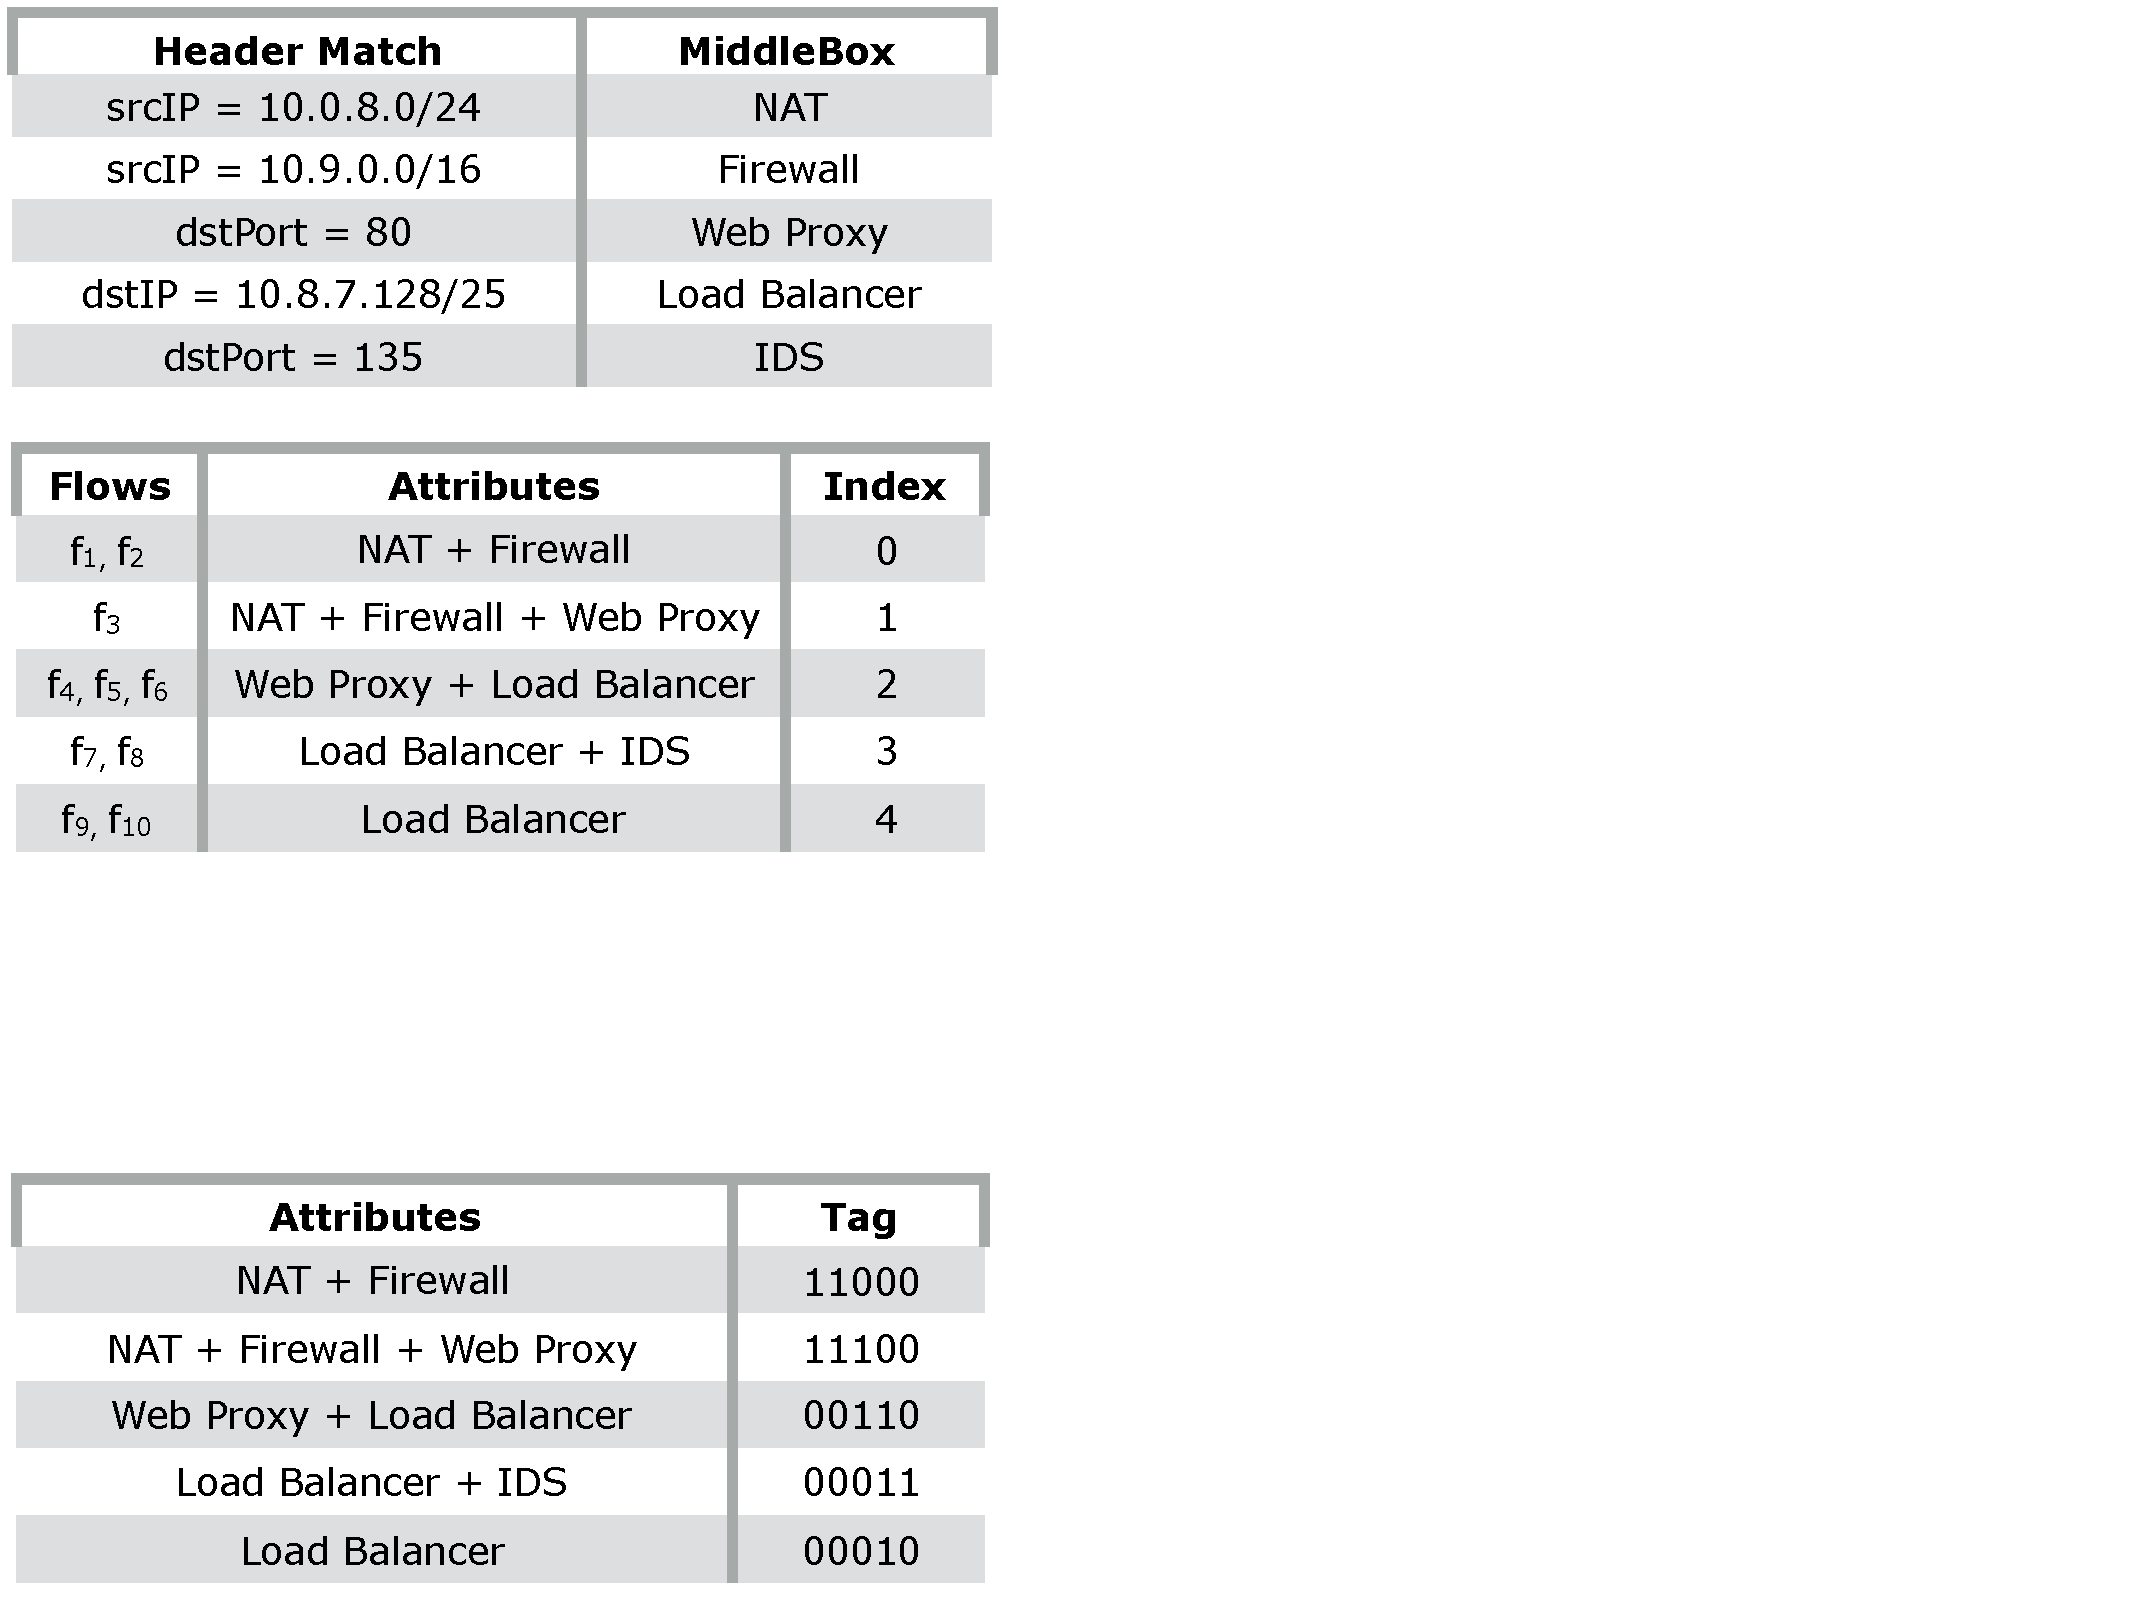
\includegraphics[trim={0 12cm 19cm 0}, clip, width=\linewidth]{figures/mbox_path_example3}
\end{subfigure} 
\end{minipage} 
\caption{In this example, we have a policy that defines traffic which must flow through subsets of five middleboxes. The first table shows which header fields trigger each middlebox, and the second table shows some combinations we may see in network traffic. }
\label{fig:mbox_policies}
\end{figure}

We mentioned flat index labels and their applications in the introduction. In this section, we will discuss flat labeling schemes, their implementation in commodity switches, and their limitations. We will use these limitations as motivations for new labeling schemes which take advantage of recent changes in commodity switches.

\subsection{Match-Action Tables}
In order to understand how our result came to be, we must first explain what features commodity switches have supported and how they have evolved in recent years. Commodity switches traditionally use match-action tables for determining how to handle packets. Match-action tables are populated by \textit{forwarding rules} at runtime. A forwarding rule $<M, A>$ is made of a set matching conditions $M = [m_1, m_2, ..., m_C]$, and an action $A$ to apply to a packet $P$ if the matching conditions are met, or in other words if $M(P) = true$. Actions include dropping a packet, rewriting a header field, or forwarding the packet out a specific port. Each matching condition $m_i = [field, type, S]$ is comprised of a packet header field designation ($field$), a matching type ($type$), and a match string $S$. $field$ is the name of the header field the match string will be compared to. Each match string is a ternary string $S \in \{0,1,*\}^{W_field}$, where $W_field$ is the width of the designated header field. $Type$ specifies how $S$ is compared to the header field. There are three types of matches in commodity switches:
  \begin{itemize}
  \item{\textbf{Exact Matching:} $S \in \{0,1\}^{W_field}$ is a binary string, and $M(P) = true$ if $S == P[field]$.}\\
  \item{\textbf{Longest-Prefix Matching:} $S$ is a ternary string, where the first $x$ characters are drawn from $\{0,1\}$ and the remaining $W_field - x$ are the character $*$. $M(P) = true$ if the first $x$ characters of $S$ exactly match the first $x$ characters of $P[field]$, and there is no other longest-prefix match forwarding rule such that the first $y$ characters match for some $y > x$.}\\
  \item{\textbf{Wildcard Matching:} $S \in \{0,1,*\}^{W_field}$ is any ternary string. $M(P) = true$ if, for every $0 \le i < W_field$, either the $i^{th}$ character of $S$ is $*$, or the $i^{th}$ character of $S$ exactly matches the $i^{th}$ character of $P[field]$.}
  \end{itemize}
  
  Until recently, switches have been designed with a single matching type in mind for each supported field. For the vast majority of fields, this matching type is exact matching, with the notable exception of longest-prefix matching for IPv4 address fields. Consequently, any innovation in networking research which repurposes a less-used packet field for carrying information across the network is forced to treat a single field as a single piece of information. If the researcher wishes to carry multiple pieces of information, either multiple fields must be used, or these pieces must somehow be multiplexed into a single value. The former approach is undesirable, as researchers often have a hard enough time choosing even a single field to repurpose. We will discuss the latter approach in more depth in the next section. 
  
  However, with recent changes to commodity switches, such as new features supported by OpenFlow 1.3 switches[cite:OF13] and flexible protocol-independent switches[cite:P4], we are no longer forced to work within the constraints of how hardware vendors have expected packet headers to be used. Specifically, we are able to define our own fields and apply longest-prefix or wildcard matching to fields which have previously only supported exact matches. If researchers wish to attach multiple dimensions of information to a packet, multiplexing into a single field.... PAUSING FOR READING GROUP

\subsection{Forwarding Equivalence Class Tagging}
  
In the introduction, we briefly mentioned existing index tagging schemes and their limitations. We will refer to these schemes as \textit{flat tagging} schemes, because each tag can be thought of as a single, unstructured index.  We will now go into a more detailed explanation of such schemes. A flow of packets is defined by a combination of header fields that each of the packets has in common. Each combination of header fields can imply a set of attributes which are revealed by classification, such as a set of routes the flow may take, network nodes the flow must traverse, or characteristics of the sending/receiving hosts. Figure \ref{fig:mbox_policies} shows the concrete example of service chains. Each flow has a set of middleboxes it must traverse, and this set is determined by the classification rules in the first table.

Network nodes must be aware of these attributes to correctly implement a policy. In our example, not all flows should traverse the NAT. To determine which flows to route to the NAT, each node could re-perform classification. However, the number of rules may be prohibitively large to install on each node. 

One solution for avoiding re-classification is to compile the results of classification into a short \textit{tag} and attach this tag to each packet. Switches may then read these tags to discover the attributes. If we maintained global knowledge of every distinct set of attributes seen in the network in an array, we could then use the array indices as packet tags and provide each switch with the index-to-attributes mapping. This mapping is shown in the second table of figure \ref{fig:mbox_policies}. Switches can then recover all attributes by reading the tag. 

%However, a good format for these digests which minimizes both the digest size and read operation complexity is unclear. 

This tagging scheme is optimal in tag width, because it uses the minimum number of bits required to convey which attribute set is attached to the flow. However, optimal width comes at the cost of attribute reading complexity. If a switch wishes to make a decision based only upon attribute $x$, it must compare each tag to the indices of every set that contains attribute $x$. In our example, the Load Balancing middlebox is present in three tags, so switches must compare the packet's tag to each of the three tags to determine if the middlebox is in the attribute set. In general, if the number of attribute sets is large enough, this tagging scheme may barely improve upon the memory used by performing re-classification at every switch!

%Flat tagging is a format which optimally minimizes digest size at the cost of read complexity. The result of every classification is a set of indirect attributes, which has an exponential number of possibilities, but for many applications only a small number of unique sets are seen. 



% to attach the result of classification as a digest to the headers of every packet in the flow. 

%assign a t, after classifying a flow, to attach a tag to each packet in the flow which contains the indirect attributes. 


\subsection{Attribute-Carrying Tags}

\begin{figure}[t!] 
\begin{minipage}{1\linewidth}
\begin{subfigure}[c]{0.96\linewidth}
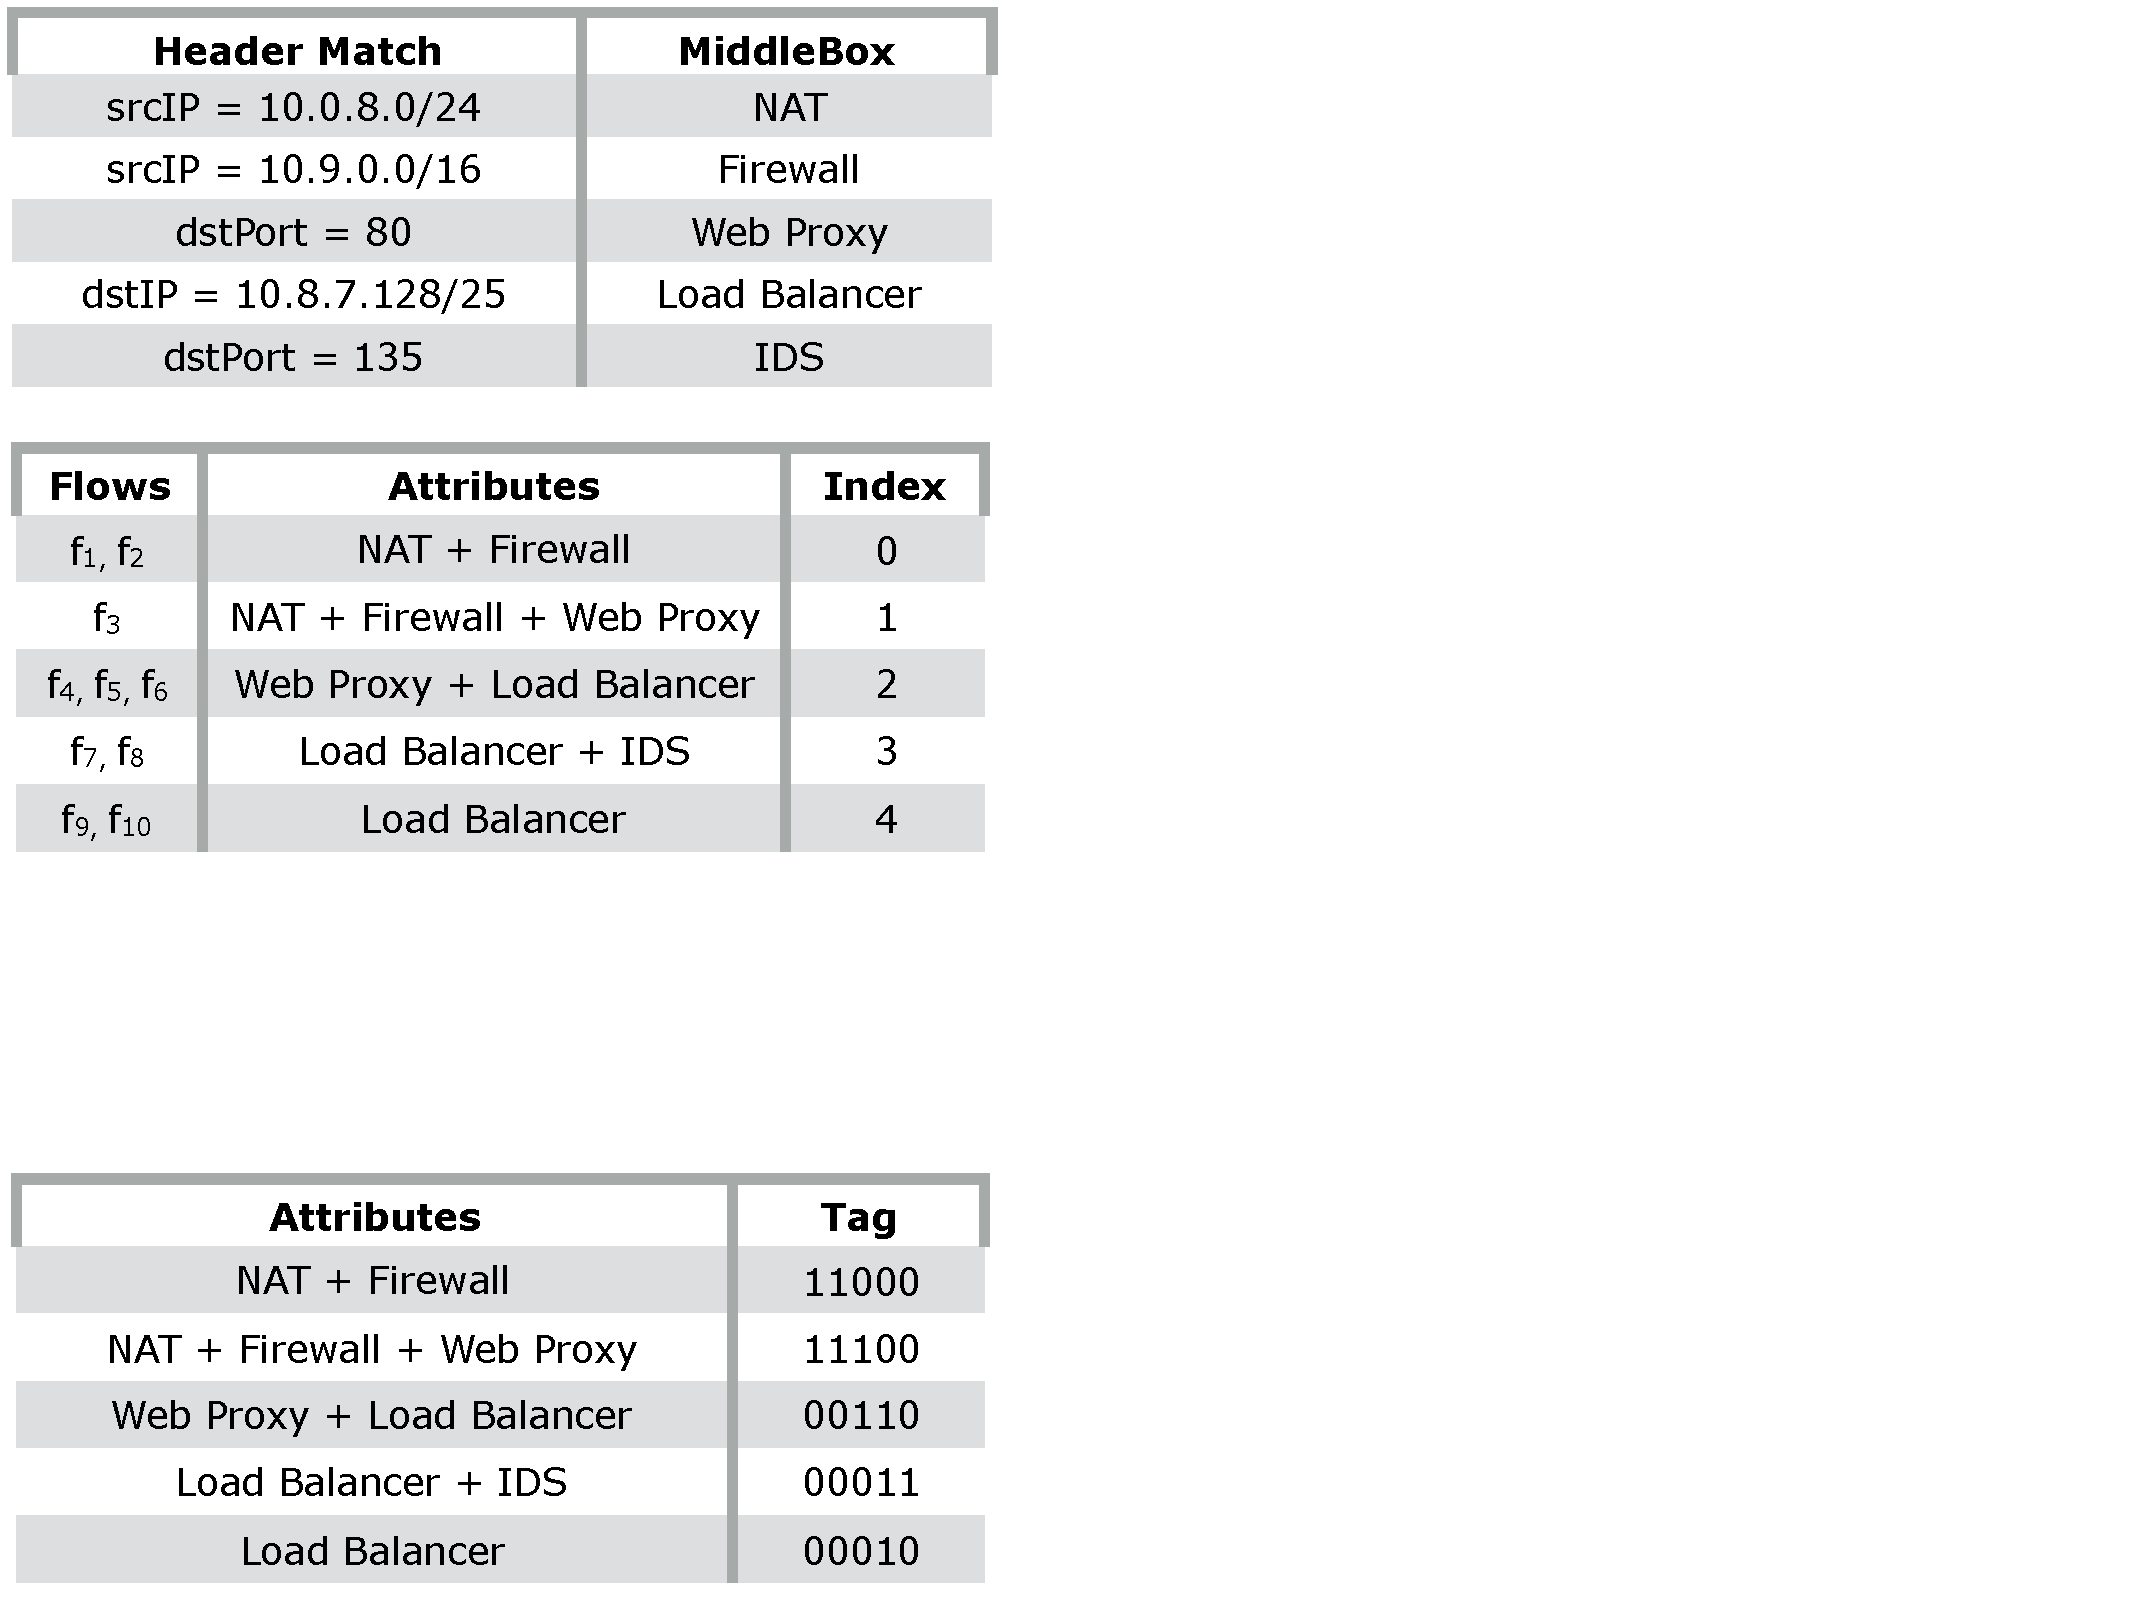
\includegraphics[trim={0 0 19cm 19.5cm}, clip, width=\linewidth]{figures/mbox_path_example3}
\end{subfigure} 
\end{minipage} 
\caption{A simple attribute-carrying tag format for the service chaining example. Each middlebox is mapped to a bit in the tag, and that bit is 1 if the middlebox must be traversed.}
\label{fig:att_tags}
\end{figure}

Attribute reading need not be so complex, though. If we do not require optimal tag width, we can construct tags such that the attributes are more quickly read. Figure \ref{fig:att_tags} shows such a construction for service chains, with tags as bitfields. Each attribute can be read using a single wildcard match, but the tag width is equal to the number of middleboxes. It is interesting to note that when each bitfield tag is viewed as an integer, it can still be thought of as an index into a implicit table of all possible attribute sets. 
%%%%%%%%%%%%%%%%%%%%%%%%%%%


\subsection{Motivating Applications}
There are many situations where a forwarding equivalence class is characterized by a distinct set of attributes, and where the switches could benefit from being able to read these sets using a small amount of memory. To motivate our solution, we will present three/four such settings. 

\subsubsection{Software-Defined Internet Exchange Points}
Consider the example of an Internet Exchange Point (IXP) with support for SDN policies. At such an IXP, connected networks may wish to apply SDN policies to their traffic as it enters the exchange point. If these policies were not present, all traffic from some network $P$  to some destination IP prefix $d$ would be directed to the BGP default next-hop for $d$ as decided by $P$. In the presence of SDN policies, however, traffic may be redirected to take a next-hop which differs from the BGP default next-hop. For correctness, this redirection must be to a next-hop which has announced a route to $d$ , and $P$'s policies must take this into account. If it were possible to attach to each packet leaving $P$ the set of next-hops which have advertised $d$ to $P$, policies could check for the presence of a next-hop in the set before rerouting the packet to that next-hop. 

\subsubsection{Service Chaining}
For another example, network operators often desire that network traffic be directed through a series of middleboxes, such as load balancers or firewalls. Such middleboxes can provide security and performance guarantees for the network's users. However, each flow may need to be directed through a different chain of middleboxes. In this case, the set of attributes which define an equivalence class would be a chain of middleboxes. Switches could check for the presence of a middlebox attribute in the FEC tag and, if present, forward that flow towards the nearest matching middlebox. This could be accomplished with an MPLS label stack, but middleboxes do not necessarily understand or preserve MPLS labels. 

\subsubsection{Host Attributes for Network Policies}


\subsubsection{Multicast and Anycast}
For another example, consider the case of anycast. In traditional anycast, many receivers are identified by the same address, and each anycast packet simply chooses the nearest receiver according to some distance metric. There is no flexibility for selecting arbitrary subsets of hosts without applying the same identifier to the subset of receivers. We envision the potential for a more flexible local area network anycast, where each packet can be mapped to an arbitrary subset of hosts, regardless of their addresses. If it were possible to tag each packet during classification with a list of host identifiers, switches could read this list and pick the nearest for forwarding.
\section{Encoding Attribute Sets}
\label{sec:flextag_encoding} 
The simplest way to encode a set of attributes is a bitmask with one
bit for each attribute, at the expense of large tags.  In this
section, we present a concise encoding that uses multiple smaller
bitmasks on different subsets of attributes, at the expense of
slightly larger rule tables.  We also present an algorithm for
computing the concise encoding.

\subsection{Strawman: Bitmask Tags}

We will now present a strawman tagging scheme which always achieves optimum switch memory usage by using wildcard matches.
If there are $N$ possible attributes to encode in a tag, construct a tag of length $N$: 
the $i^{th}$ bit corresponds to the $i^{th}$ attribute. When the packet is classified
and the tag is attached, the $i^{th}$ bit is set to 1 if the $i^{th}$ attribute
is present for that flow, and 0 if it is not. As a result, if we wish to test for
the presence of attribute $x$, we need only check that $x$'s bit is 1 in the
metadata, rather than exact matching on every tag that contains
$x$.

This approach is a strawman because the tag is of width $N$, and $N$ can be quite large.
Although we criticized flat tagging for using too much switch memory, 
flat tagging only needed tag width logarithmic in the number AECs. We have just traded an extreme in memory
usage for an extreme in tag width. It would be ideal to find some middle ground.
In general, any tagging scheme must simultaneously consider three different metrics:

\begin{enumerate}
\item \textbf{Tag Width:} Tags should not be too wide, to avoid wasting packet-header space.
Tags should be able to either be inserted into small repurposed header fields or contribute little size to custom packet headers. 
\item \textbf{Switch Memory:} The amount of memory required to decode attributes from any tag should be able to easily fit in modern commodity switches rule tables.
\item \textbf{Churn:} Normal network events should not cause the encoding scheme to undergo too many changes.
\end{enumerate}
%It is these metrics by which we will evaluate our solution.
%%%%%%%%%%%%%%%%%%%%%%%%%%%


%To understand the problem, let us consider a
%simple example for the case of attaching lists of anycast hosts to a packet. Say
%that there is a local area network with five hosts $H = \{h_1, h_2, h_3, h_4,
%h_5\}$, and each packet that arrives will be classified as anycasting to one of
%four possible host sets: $s_1 = \{h_1, h_2\}$, $s_2 = \{h_1, h_2, h_3\}$, $s_3 =
%\{h_1, h_3\}$, or $s_4 = \{h_3, h_4, h_5\}$. In a flat tagging solution to this
%problem, each unique set will be assigned a single tag, and thus a packet which
%can be forwarded to the $i^{th}$ set will receive the $i^{th}$ tag. Now, for an
%intermediate switch to determine, using exact tag matches, if a packet can be
%forwarded to host $h_1$, it must check whether the packet has been assigned to
%$s_1, s_2,$ or $s_3$. The number of entries required is proportional to the
%number of sets which contain $h_1$, in this case 3. In the worst case $h_1$
%would be a member of almost every group, and testing for $h_1$ would required a
%number of checks linear in the number of tags. 

\begin{figure}[t!] \begin{minipage}{1\linewidth}
\begin{subfigure}[b]{0.96\linewidth} 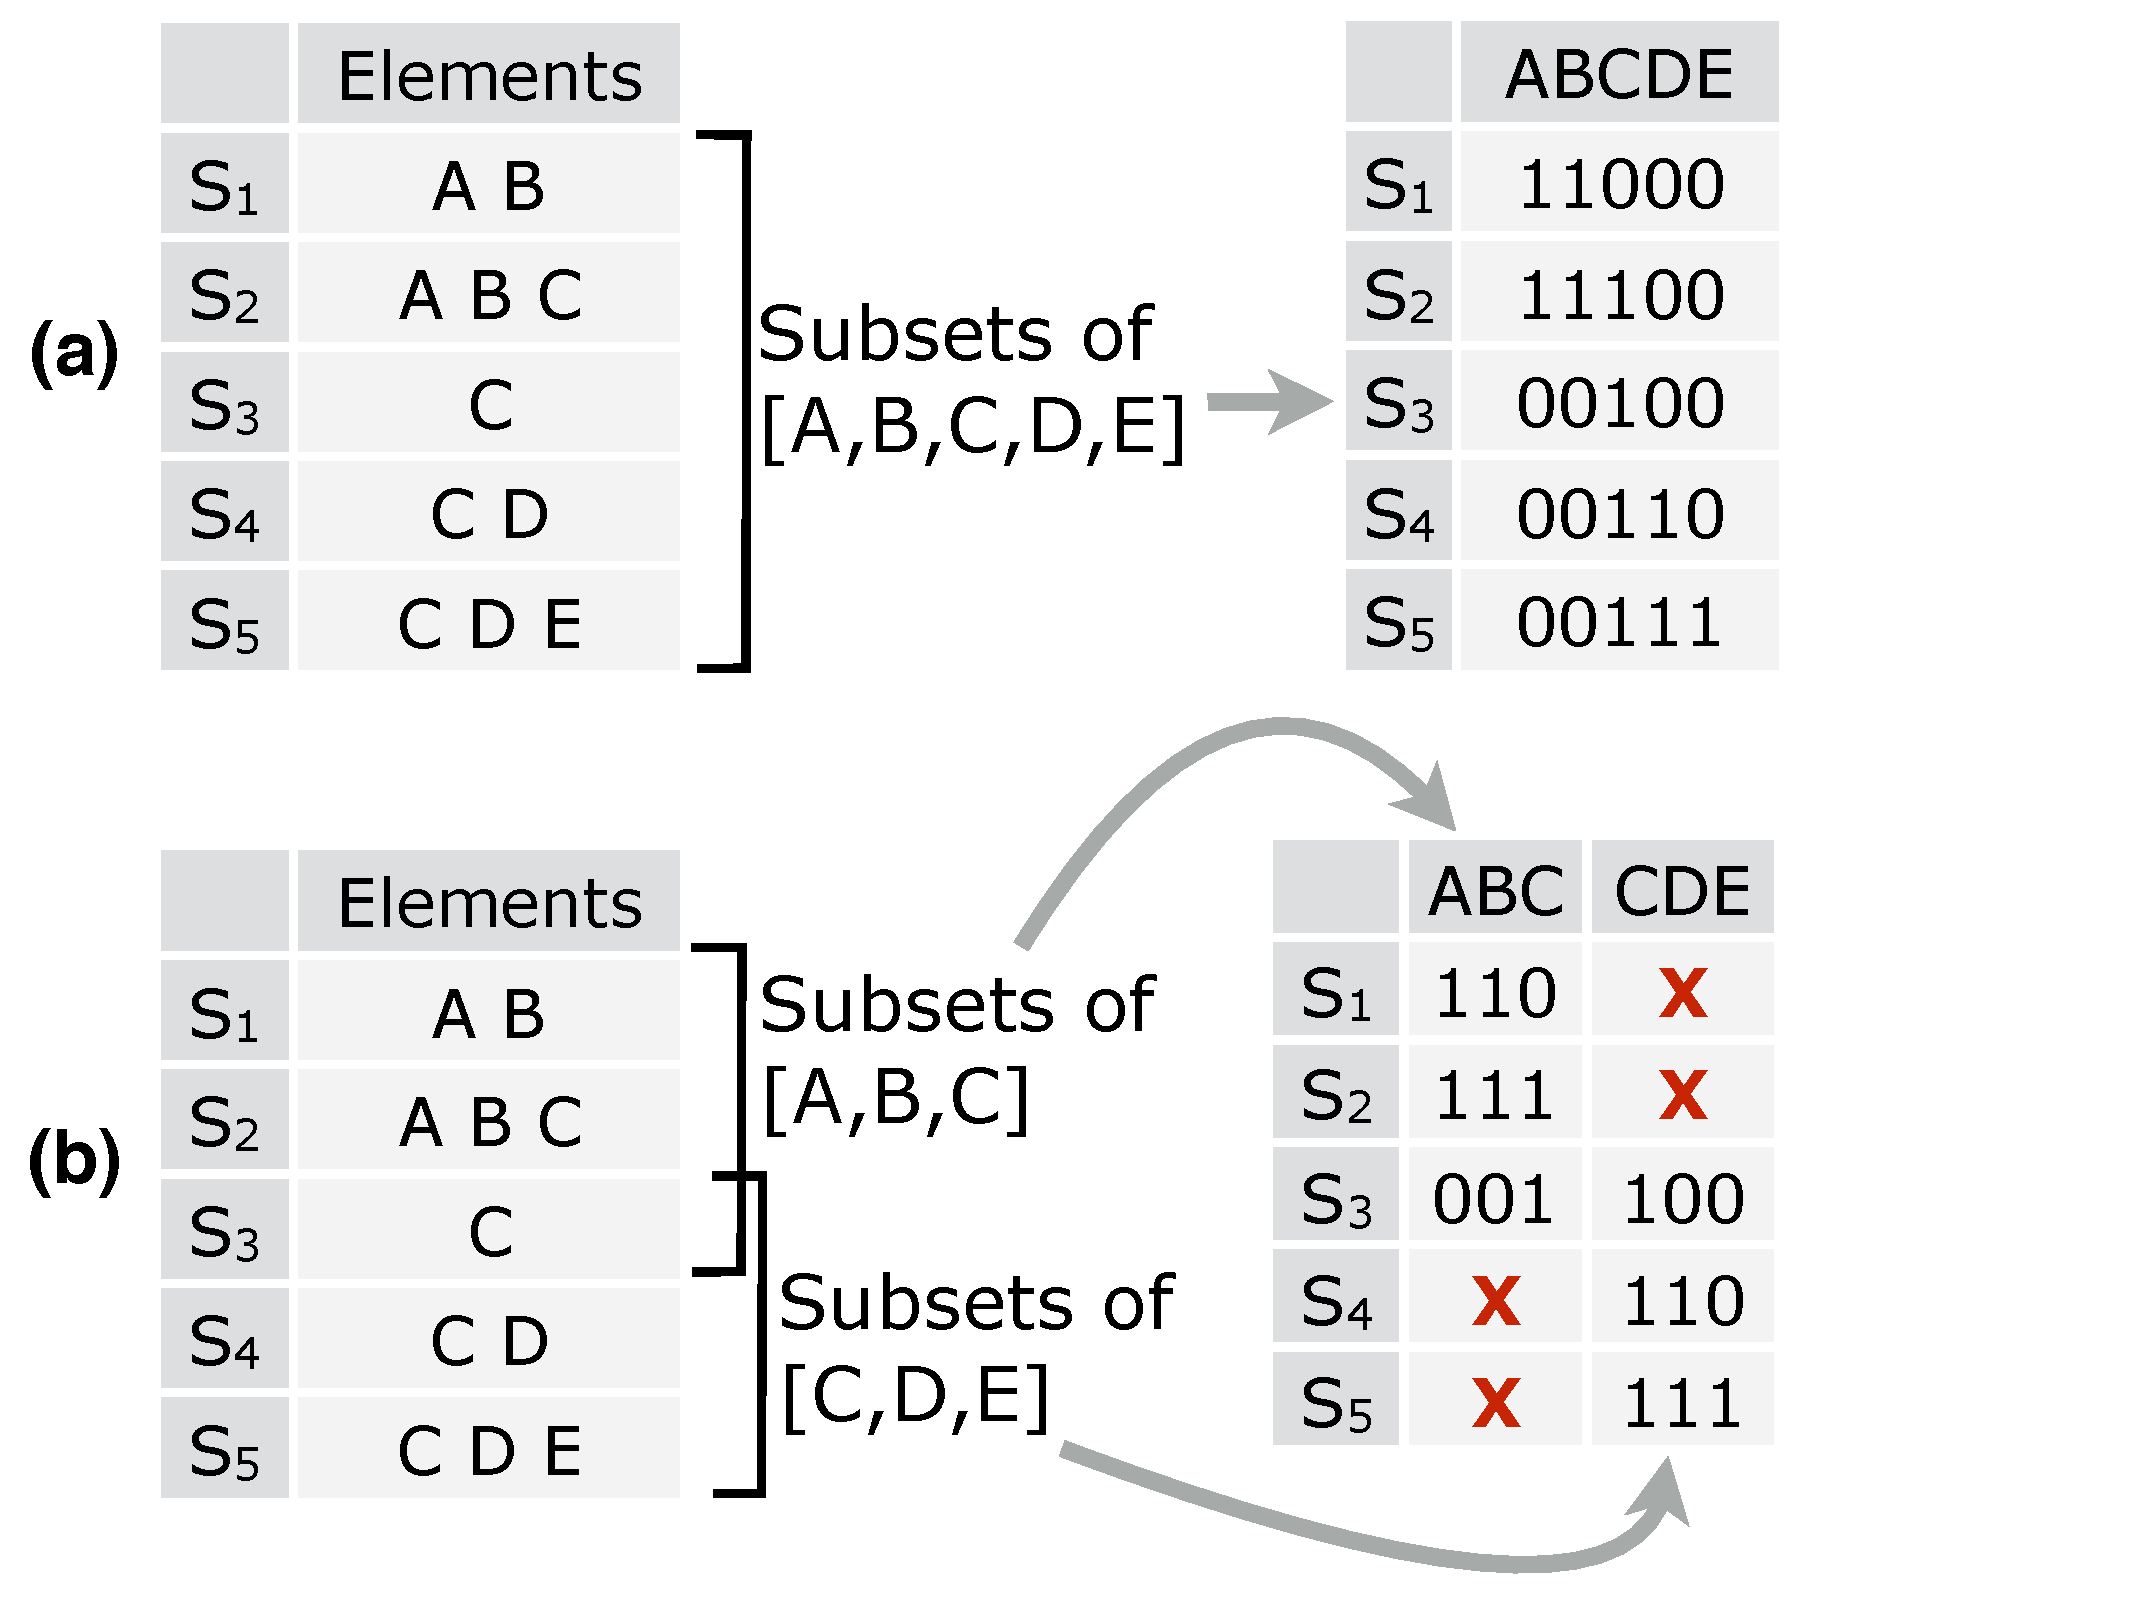
\includegraphics[trim={0 0 5.5cm 0}, clip,
width=\linewidth]{figures/masking} \end{subfigure}
\begin{subfigure}[c]{0.96\linewidth} 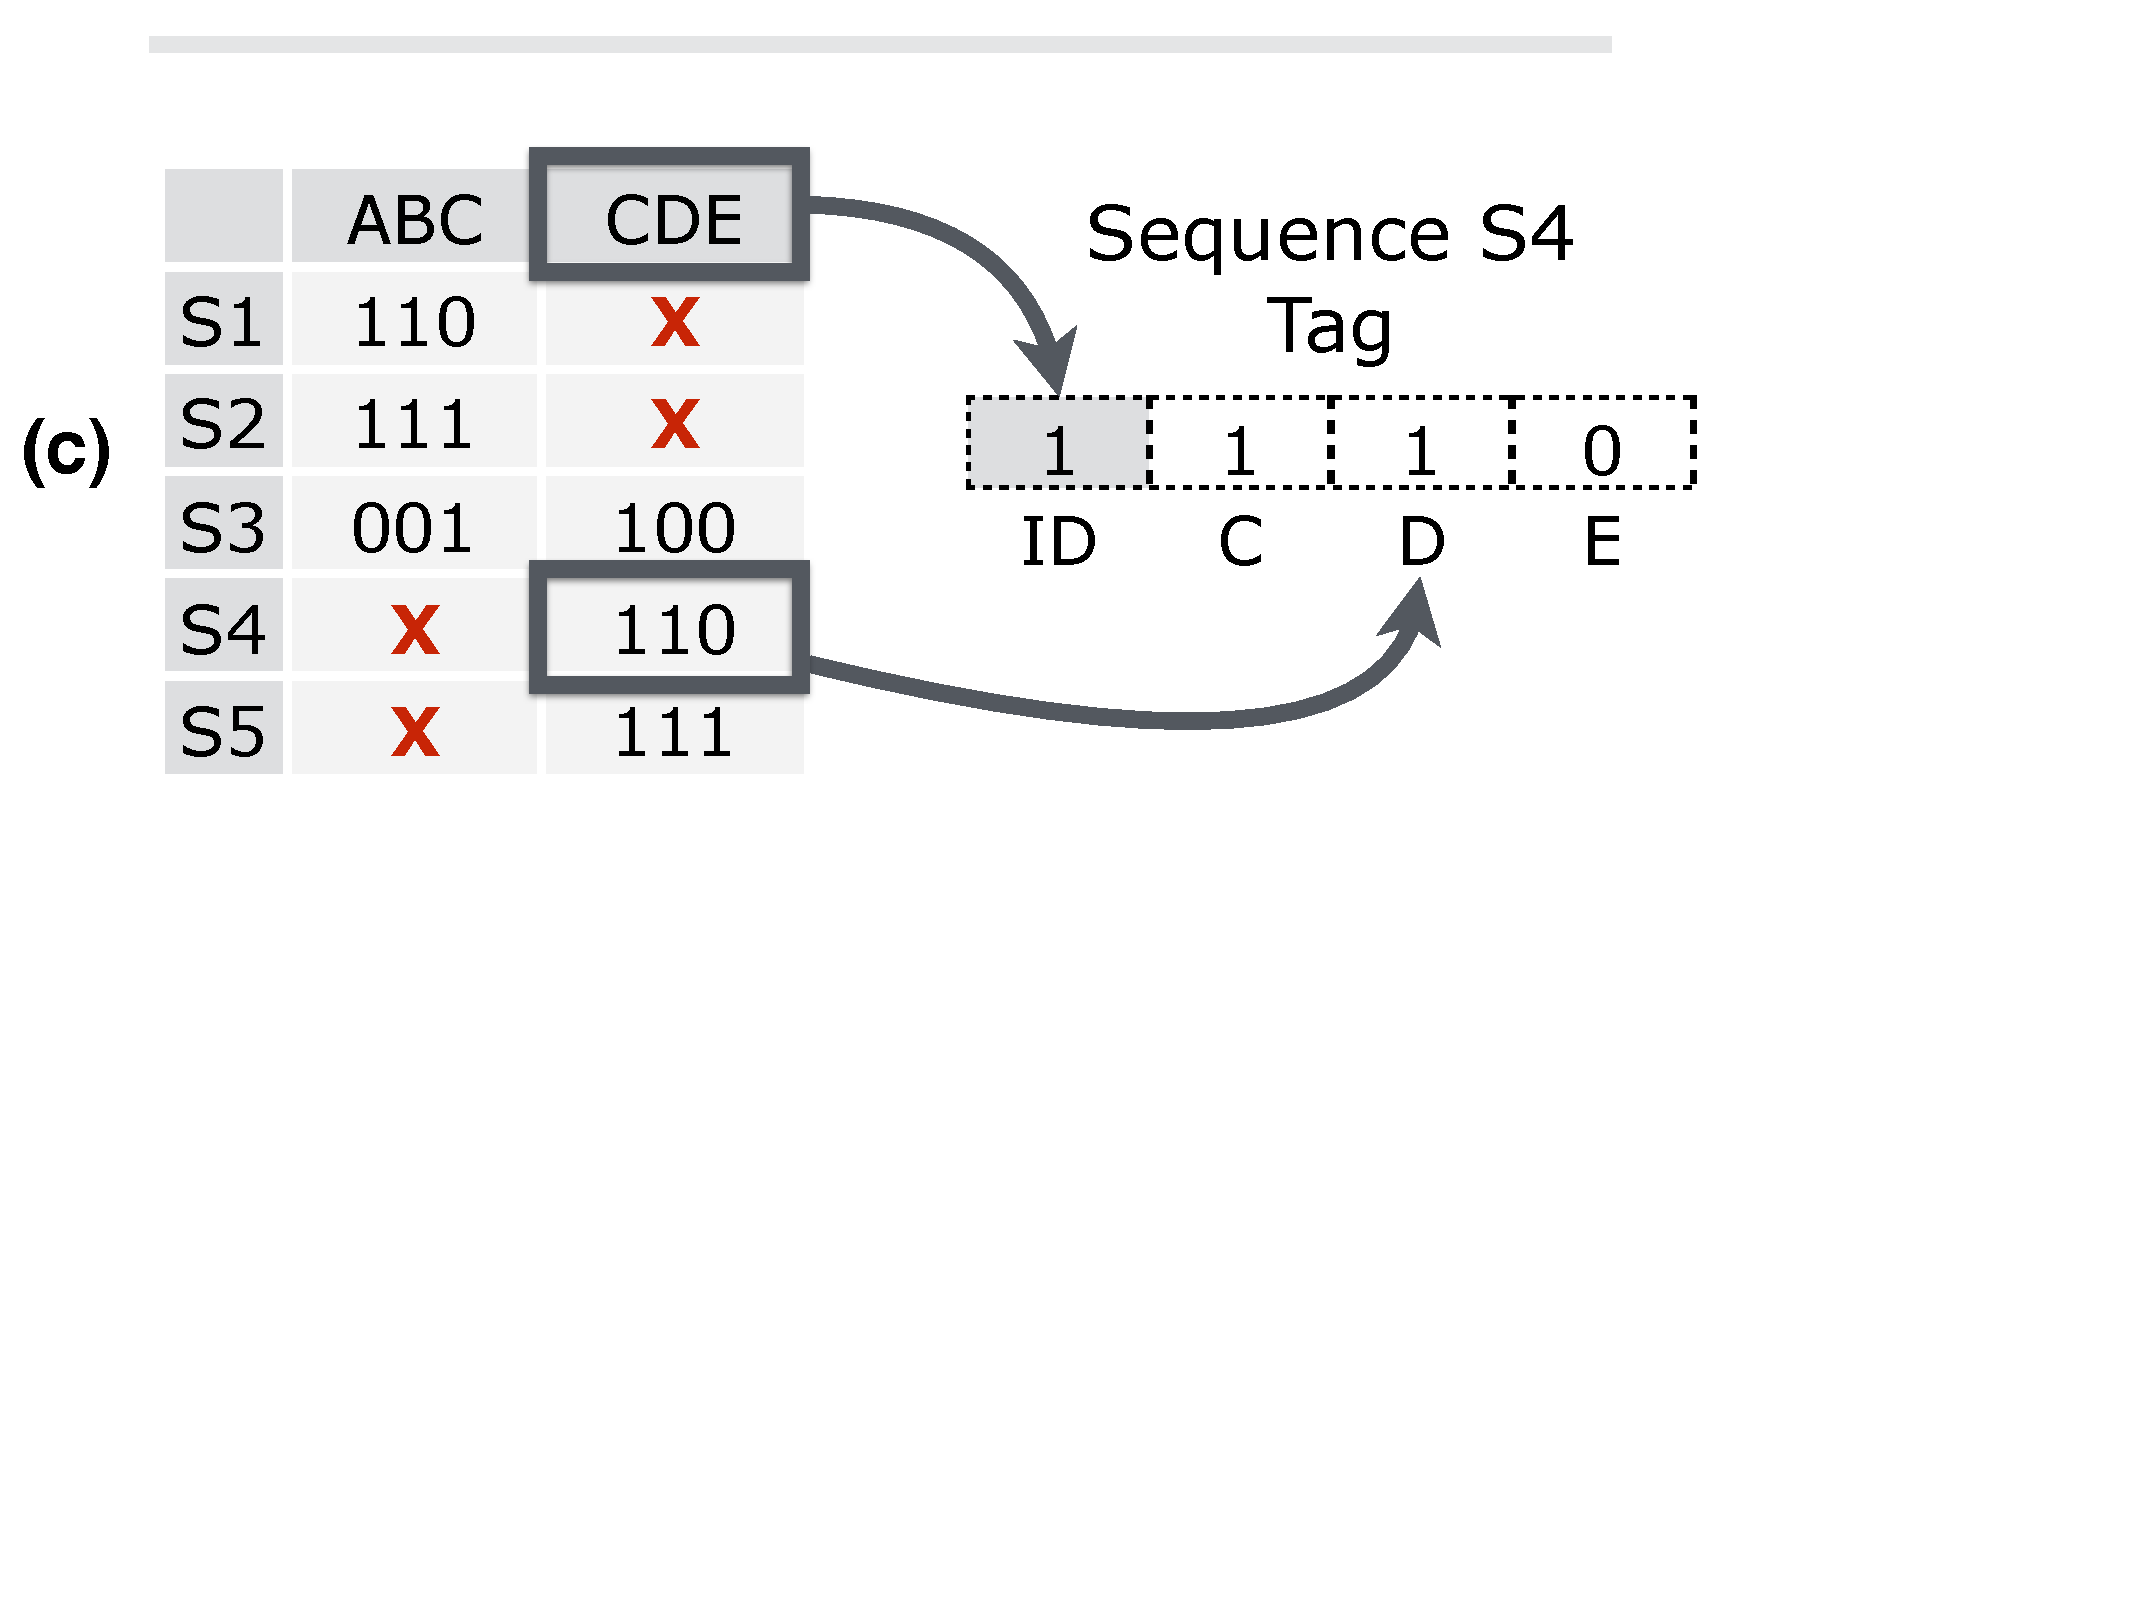
\includegraphics[trim={0 13cm 5.5cm 0},
clip, width=\linewidth]{figures/making_metadata} \end{subfigure} \end{minipage}
\caption{Two different ways to recover attribute sets.
In (a), the sets are recovered by masking over $[A,B,C,D,E]$. In (b), the sets
are recovered by masking over either superset $[A,B,C]$ or set $[C,D,E]$. An X
denotes that the set cannot be fully recovered by masking over the given set.
(c) shows how the matrix in (b) can be mapped to tags.}
\label{fig:masking} \end{figure}

\subsection{Multiple Smaller Subsets of Attributes}
\label{ssec:mset}
%%%
%%% Strawman
%%%
In the strawman solution of a simple bitmask, the tag has one bit for
each boolean attribute.  For example, Figure~\ref{fig:masking}(a)
shows multiple attribute equivalence classes ($S_1$-$S_5$) that each
correspond to a different subset of five attributes ($A$-$E$).  The
network policy determines which traffic has which attributes, and
which combinations of attributes can hold together.  For example, all
packets with attributes $A$ and $B$ true, and $C$, $D$, and $E$ false,
belong to attribute equivalence class $S_1$, and can be encoded with
the bitmask ``$11000$''.  Certain combinations of attributes may not
occur for any traffic (e.g., attributes $B$ and $D$ are never true
together, though both can be false as in $S_3$).  A single rule can
test for any combination of attributes (e.g., comparing a tag to
``1*1**'' identifies whether attributes $A$ and $C$ hold, without
caring whether $B$, $D$, or $E$ hold).  However, when the number of
attributes is large, a bitmask tag becomes quite large.

%%%
%%% Concise encoding example in the figure
%%%
Our more concise encoding identifies groups of attributes that
commonly appear together, and creates one shorter bitmask for each
such group.  In the example in Figure~\ref{fig:masking}, attributes
$A$, $B$, and $C$ commonly appear together, as do $C$, $D$, and $E$,
leading to two groups.  The right side of Figure~\ref{fig:masking}(b)
shows how each attribute equivalence class can be encoded as a bitmask
on $[A,B,C]$, $[C,D,E]$, or both.  To differentiate between the two
groups, the tag can include a one-bit group identifier (e.g., a $0$
for $[A,B,C]$ and a $1$ for $[C,D,E]$), as shown in
Figure~\ref{fig:masking}(c).  The result is a four-bit identifier
where, for example, $S_4$ with attributes $C$ and $D$ is encoded as
$1110$.

%%%
%%% Slightly larger rule table
%%%
The forwarding rules can match on attributes by considering both the
group identifier and the associated bitmask.  For example, a switch
could test for attribute $D$ by matching on (i) group $1$ and (ii) the
$D$ bit in group $1$'s bitmask.  Thus, the rule would have a match of
``$1*1*$''.  However, some attributes appear in multiple groups, such
as attribute $C$ in the example.  The switch can use two rules to test
for $C$: (i) ``$0001$'' for group $0$ and (ii) ``$1100$'' for group
$1$.  Thus, our encoding scheme slightly increases the forwarding
table size over the simple bitmask scheme, but only by one rule in
this example.

\subsection{Computing Concise Encodings of Sets}
\label{ssec:merge}
%%%
%%% Computing the initial groups
%%%
The tag and rule-table sizes depend on the quality of the encoding.  A
natural starting point is to have one group for each attribute
equivalence class (e.g., $[A,B]$, $[A,B,C]$, $[C]$, $[C,D]$, and
$[C,D,E]$), at the cost of a large group id.  A simple optimization is
to remove any group with attributes that are a \emph{subset} of
another group (e.g., removing $[A,B]$ and $[C]$ that are subsets of
$[A,B,C]$, and removing $[C,D]$ that is a subset of $[C,D,E]$).  In
the simple example, this heuristic results in the two groups
($[A,B,C]$ and $[C,D,E]$).  However, in larger examples, this
heuristic could still result in too many groups. Instead, we use the
set of groups ($\SS$) produced by the heuristic as an input to an
algorithm for optimizing the selection of groups.

\begin{algorithm}
\DontPrintSemicolon
\KwData{Groups $\SS$, Attribute Test Counts $\{q_k\}$, 
  Tag Width Limit, $W_{max}$, Tag Width Calculator $W()$.}
\KwResult{Groups $\SS$ with minimal rule-table size.}
\Begin{
\While{$|\SS| > 1$}{
      	$bestPair \gets (None, None)$\;
      	$bestGain\gets 0$\;
      	\For{$(s_i, s_j) \in \SS\times \SS$}{
      		$\SS_{temp} \gets (\SS-\{s_i, s_j\}) \cup \{s_i\cup s_j\}$\;
      		\If{$W(\SS_{temp}) \le W_{max}$}{
      			$gain \gets \sum_{k \in s_i\cap s_j}q_k$\;
      			\If{$gain > bestGain$}{
      				$bestGain \gets gain$\;
      				$bestPair \gets (s_i, s_j)$\;
      			}
      		}
      	}
      	\If{$bestPair = (None, None)$}{
      		\textbf{break}\;
      	}
      	$(s_a, s_b) \gets bestPair$\;
      	$\SS \gets (\SS-\{s_a, s_b\}) \cup \{s_a\cup s_b\}$\;
      }
      \textbf{return} $\SS$\;
}
\caption{Greedy Memory Minimization\label{alg:memory_min}}
\end{algorithm}

%%%
%%% Benefits of merging groups
%%%
Our algorithm iteratively merges pairs of groups, to minimize the
rule-table size while staying within some limit $W_{max}$ on the tag
size.  Suppose a switch has $q_a$ clauses that test whether attribute
$a$ is true, and the attribute appears in $k_a$ groups.  Then, the
switch would require $q_a \cdot k_a$ rules to test for that attribute.
Merging two groups can reduce the number of rules, but possibly
increase the tag size depending on the number of attributes the two
groups have in common.  Suppose $\SS = \{s_1, s_2, \dots, s_N\}$,
where group $s_i$ is a subset of attributes.  Replacing any pair of
groups $\{s_i, s_j\}$ with their union $s_i\cup s_j$ would decrease
the number of rules by $\sum_{a \in s_i\cap s_j}q_a$ because every
attribute $a$ in the intersection of the two groups would appear in
one fewer group after the merge.

%%%
%%% Greedy algorithm
%%%
We can extend this observation to a greedy algorithm that repeatedly
identifies the pair of groups to merge that maximally decreases the
number of rules without exceeding the $W_{max}$ tag size.
Algorithm~\ref{alg:memory_min} shows the pseudocode.  The algorithm
takes as input a set of attribute groups $\SS = \{s_1, s_2, \dots,
s_N\}$, the attribute test counts $\{q_k\}$, a maximum tag width
$W_{max}$, and a tag-width calculator $W()$.  The tag-width calculator
determines the number of bits in the tag, given the current set of
groups $\SS$.  We present closed-form equations for the tag-width
calculator later in \S~\ref{sec:identifiers}.
\jrex{what is the computational complexity of the algorithm? 
Should we stress that the algorithm can stop at any time -- the
longer you run the better, but you don't have to run to completion.}


%

\section{Optimization Memory and Tag Width}

%In each motivating use case we have given, traffic equivalence classes are characterized by unique sets of attributes. We claim that we can construct a tag for each equivalence class which switches may use to determine the class's attributes using some set of wildcard rules. In this section, we will go over what those rules look like.

%In wildcard rule tables, a rule is a $<match, action>$ pair, where $match$ is a wildcard string which is compared to the packet header, and $action$ is the action the switch takes if the string comparison returns true. Match strings are strings over the alphabet $\{0,1,*\}$, where 0 and 1 are specific bit values, and $*$ denotes "don't care". Given a packet header consisting of bits $\{h_1,h_2,\ldots,h_n\}$ and a wildcard string $\{w_1,w_2,\ldots,w_n\}$, they are said to match if for every $i$, either $h_i = w_i$ or $w_i = *$. 

It is our goal to construct a tag for each FEC such that if an attribute exists across many sets, a single set of rules can determine if that attribute is true for any tag. Additionally, we wish for the maximum width of any tag to not be too large, and for the number of rules required by all attribute testing to be minimized. 

For each attribute $i$, a number of attribute tests $t_i$ will be performed. If $r_i$ rules are required to perform one test, then there are $t_i\cdot r_i$ rules associated with attribute $i$. The total number of rules required by a tag assignment is thus $\sum_i{t_i\cdot r_i}$. 


In the introduction, we discussed flat tags and attribute-carrying tags. We noted that flat tags optimally minimize tag width, and we gave a simple example of an attribute-carrying bitfield tag that minimized the memory used by switches. Each of the two examples minimized one desirable property while ignoring another. In the previous section, we devised a new format for attribute-carrying tags which achieves some middle-ground, giving better widths than bitfield tags, and better memory usage than flat tags. However, we did not discuss how to encode the given attribute sets into this format. 



%For this scheme of attaching information sets to packets to be feasible with commodity switches, it must be possible for membership testing to be implemented in the forwarding tables of switches. In switch TCAM tables, rules are are comparisons between a fixed string and the packet header, where the fixed strings are over the alphabet $\{0,1,*\}$. $0$ and $1$ are specific bit values, and $*$ denotes "don't care". We say that a packet header matches a string if for every bit in the header, either the bits are equal or one is a wildcard. Example usages include exact matches (strings with no wildcards), prefix matches (strings that end in wildcards), and reading of individual bits (strings with only one non-wildcard). 


 %(TODO: cite some tagging works like flowtags and the original SDX?) have solved the problem of associating packets with information sets by generating a tag for each unique information set and repurposing one of the fields in the header for the tag. In the FlowTags work, each middlebox path had its own set of tags, which could fit into the IP Fragment Identification field. To determine if middlebox $X$ is the next-hop, switches must compare the tag to every tag which has $X$ as a next-hop using TCAM exact matches. This can result in a TCAM entry count exponential in the number of bits in a tag. In the SDX work, each set of next-hops had a unique tag which was placed in the destination mac field. Again, to determine if next-hop $X$ is correct, the tag must be compared against every tag which contains $X$ using exact TCAM matches. 

%In both works, the number of bits required can be quite small, but membership tests are expensive, requiring rules exponential in the tag size. TCAM is a very limited resource, and it would be desirable to design tags with the goal of decreasing the number of entries required for membership testing. 

%To combat these issues, we present a compression scheme which allows
%the encoding of sequences over a large number of elements, such as service chains or lists of BGP next-hops, into a format easily queried by commodity switches. We show how, with an additional algorithm, this scheme can be used to compress both ordered and unordered sets. Finally, we evaluate our algorithms across both synthetic and real datasets, and show not only does the number of bits needed by our compression scheme compete with the number of bits needed by tags, but that that each core switch need only a constant number of entries per membership test, versus a linear number of entries for the case of flat tagging.




When encoding attribute sets into superset format, there are two different objectives to keep in mind: minimizing the number of bits required by the superset identifier and mask, and minimizing the cost of membership tests. If the goal was simply to minimize the number of bits required, we would have no bits for the mask and dedicate the entire tag to the identifier. This is flat tagging, and the number of TCAM entries required for membership tests would be maximized. If the number of bits for tagging was unconstrained, we would have no bits for superset identifier and simply have one large mask, causing each membership test to require only one TCAM entry. The problem only becomes interesting once both objectives are considered simultaneously, which we will now formalize. 

Let $\mathcal{A} = \{s_1, s_2, \dots, s_A \}$ be the list of distinct attribute sets for all seen equivalence classes, where each set $s_i$ is drawn from a universe of attributes $U = \{1, 2, \dots, N\}$. Associated with each element $j$ is a weight term $w_j$, which corresponds to the number of times attribute $j$ is read by network nodes. We are also given a hard limit on the width of equivalence class tags, denoted by $B$. 

Our goal is to construct a mapping $\mathnormal{f}$ such that 
$s_i \subseteq s_k \Leftrightarrow  \mathnormal{f}(i) = k \in \{1, \dots, Z\} $. In other words, we wish to choose a value $Z$, partition the input attribute sets into $Z$ groups, and union each group to create $Z$ supersets.

In these terms, the objective function we aim to minimize is

\begin{samepage}
$$ \min \sum_{j \in U} w_j \cdot |\{z_k | j \in z_k \}| $$

OR

$$ \min \sum_{j \in U} w_j \cdot \sum_{k \in [1\dots Z]}\mathbbm{1}_{j \in s_k} $$

Subject to

$$ \log_2{Z} + \max_{k \in [1\dots Z]}\{s_k\} \le B $$

\end{samepage}

The inner sum of the objective function denotes the number of supersets which attribute $j$ appears in. If this number is $x$, then there will be $x$ different types of tags which may contain $j$. To test for attribute $x$
This objective reflects the amount of memory which will be used by a tag set generated from the chosen supersets. 



%Where $a_j$ is the number of supersets that element $j \in U$ belongs to, and $B$ is the maximum number of bits that our tag can use. The objective function reflects the number of TCAM entries required for all membership tests. If the network tests for the membership of element $j$ $w_j$ times, and $j$ appears in $a_j$ supersets, then our approach requires $a_j w_j$ TCAM entries. 
The constraint shows that a superset construction is feasible if the identifier size plus the mask size is less than the bit constraint $B$. The identifier size is $\log_2{Z}$ if $Z$ is the number of supersets, and the mask size required is the maximum superset size, or $\max_{s_i \in S}\{s_i\}$.

%We suspect that this problem is NP-Complete for \mbox{$M > B$}, but a proof of the claim is left as future work. 

\subsection{A Greedy Algorithm}

Although the problem may be hard, we can still formulate heuristics for constructing good-enough solutions. We begin with $N$ supersets, where superset $i$ is the $i$th list wish wish to recover. This solution is, by construction, able to generate every required element list, but it may not be feasible. $N$ may be so large that the superset identifier will dominate the metadata and exceed the bit limit. This solution will also certainly require a large number of TCAM entries, as no sets have yet been combined into supersets.

In the first step of the algorithm, we delete any supersets which are subsets of other supersets. If superset $s_i$ is $[A,B,C]$, and superset $s_j$ is $[B,C]$, then there is no use for $s_j$ and it may be deleted. Deletion strictly improves the solution because any subset of $s_j$ can still be recovered from $s_i$, and the superset identifier decreases in size as the number of supersets decreases. In practice, this reduces the number of sets down from hundreds of thousands to less than one hundred.

In step two, we attempt to greedily decrease the number of bits required by our feasible solution by merging pairs of small supersets together that do not increase the maximum mask size when unioned. The idea is that this will decrease the number of sets and thus the size of the superset identifier will decrease. This step repeats until every feasible merging action would increase the number of bits required. 

In step three, we improve the remaining supersets in an iterative greedy fashion. We consider all feasible mergings of pairs of supersets, where a feasible merge is a union of the two supersets which does not result in the new mask size exceeding the bit limit. The \textit{benefit} of a merging is the decrease in the number of flow rules which will result
from the merge. The decrease is the sum of the weights of each participant which appears in the intersection of the two supersets, where the weight is the number of flow rules in which the participant appears. This is because after a merging of two sets, every participant which appeared in the intersection now appears one less time across the supersets, and thus every rule they appear in can be replicated one less time. 

With these definitions in mind, the full algorithm is as follows:

\begin{algorithm}
 \KwData{feasible supersets $S = \{s_1, s_2, \dots, s_M\}$}
 \KwResult{a list of supersets with maximally decreased rule inflation }
remove subsets from $S$\;
let $A =$ the set of merge pairs which don't increase bits required\;
\While{A is nonempty}{
  choose pair $(s_i, s_j) = a \in A$ with smallest union\;
  merge sets $s_i$ and $s_j$\;
  update $A$\;
 }
let $A =$ the set of feasible merge pairs\;
remove any subsets from
\While{A is nonempty}{
  choose $(s_i, s_j) = a \in A$ with greatest benefit\;
  merge sets $s_i$ and $s_j$\;
  update $A$\;
 }
\end{algorithm}

The loops consider all pairs of supersets in each iteration in the worst case, so they have a quadratic running time. Fortunately, the removal of subset supersets in the first step, which runs linearly on lists of supersets with high redundancy, reduces the number of supersets in such lists to a small constant, so the running time is reasonable.

%%%%%%%%%%%%%%%%%%%%%%%%%%%%%%%

%\subsection{Handling Updates}

%We have given an algorithm for computing a static solution, but not all applications will be static. For middleboxes, new paths can be introduced, and existing paths can be modified. For IXP case, routes are announced and withdrawn continuously, meaning the list of valid next-hops for many prefixes are constantly changing. Therefore, we must give a procedure for handling dynamic updates to the superset matrix.

%We begin with a feasible solution as output by our algorithm, which is a collection of supersets and a mask for each element set. We consider both cases of a new set or a modified set identically. We first generate a new superset for the new/modified set. If this new superset is a subset of an existing superset, we remove it. 

%Each time a prefix is announced or withdrawn by a participant, we consider that prefix's new list of valid next-hops. If it is still a subset of some superset, we need only update the mask. 

%If the new set is not a subset of any superset, we attempt to merge the new superset with an existing superset via the same greedy procedure we applied to the static context. If no merging is possible, we leave it as its own superset. If the introduction of the new superset causes the bit limit to be exceeded, we recompute the static solution entirely as a worst-case scenario. In our evaluations, we have found the worst-case scenario is never needed.



\section{aTag Enhancements}
We have demonstrated a tag format consisting of an attribute superset identifier and an bitmask, and presented algorithms for constructing such tags from an input list of attribute sets. However, we can do better.


\subsection{Variable Length Identifiers}
It is unlikely that all attribute supersets will be the same width, causing different tags to use a different number of bits. If we are using a fixed-width field in the packet headers for the tags, then it must be at least the size of the largest tag, and all smaller tags must be padded to the size of the largest tag. This wastes space which could perhaps be used in a more clever fashion.

\begin{figure}[t!] 
\begin{minipage}{1\linewidth}
\begin{subfigure}[c]{0.96\linewidth}
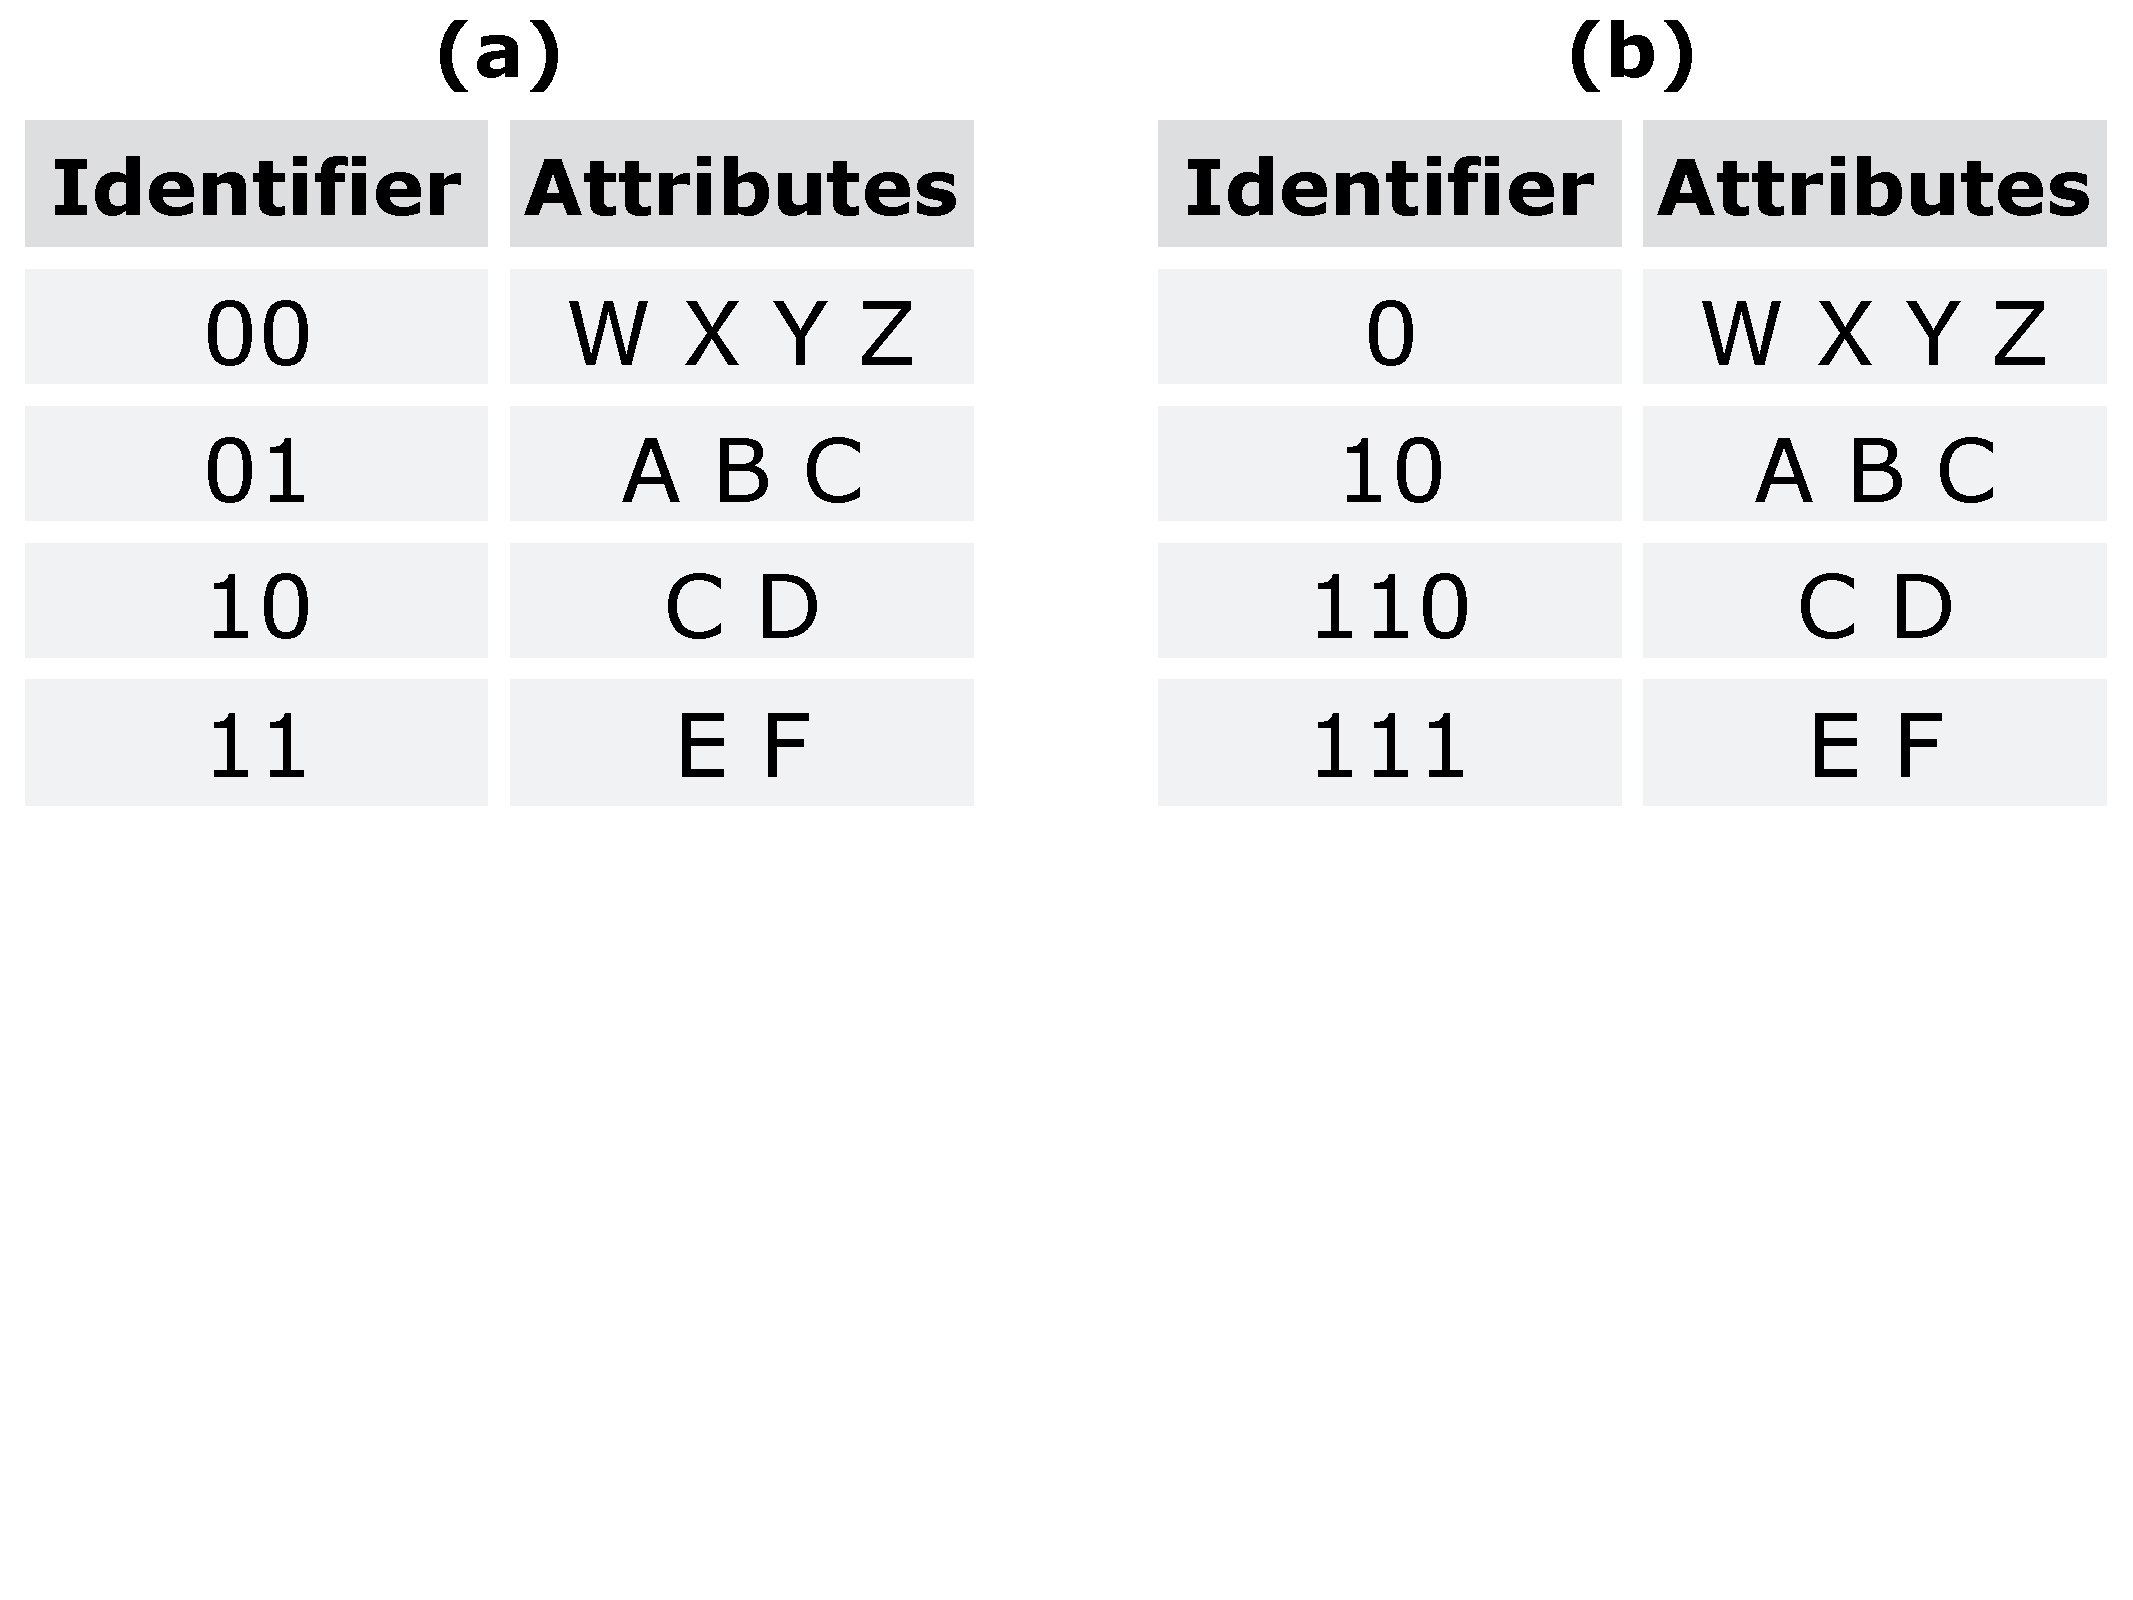
\includegraphics[trim={0 10cm 0 0}, clip, width=\linewidth]{figures/variable_identifiers}
\end{subfigure} 
\end{minipage} 
\caption{(a) shows example supersets with fixed-length identifiers. (b) shows the same supersets with variable-length identifiers. With variable length identifiers, the maximum tag width is reduced from 6 to 5 bits. }
\label{fig:variable_id}
\end{figure}

Figure \ref{fig:variable_id}(a) shows an example list of supersets, where the tag width is determined by one large superset. If the largest superset had a smaller identifier, the tag width could be decreased. We can accomplish this with the use of prefix codes. A prefix code is a set of (not necessarily equal-length) identifiers such that no identifier is a prefix of any other identifier. Figure \ref{fig:variable_id}(b) shows an example prefix code identifier assignment, which decreases the overall tag width from 6 bits to 5 bits.






\subsection{Encoding Total and Partial Orderings}
In the design of our tag format, we assumed that the attribute sets to encode have no ordering: no attribute is greater or less than any other attribute. In many cases, this is true, as in the example of encoding lists of next-hops, but this is not true for all applications. For the example of encoding paths of middleboxes, the middleboxes must be traversed in the order originally specified. As our scheme currently stands, this ordering is lost after the sequence is converted to a tag. 

\subsubsection{Total Ordering}
It is possible to impose an ordering upon the elements encoded by the tags. If the forwarding table entries which test for element membership were prioritized such that testing for element $X$ always has higher priority than testing for element $Y$, then this imposes the ordering $X > Y$ on the pair. Forwarding tables return the highest priority match, so if both $X$ and $Y$ are present in the sequence, then the test for $X$ will be the test that returns true. We can use this idea to support element ordering, so long as the element set is \textit{totally ordered}.

\subsubsection{Partial Ordering}
It may not always be the case that the attributes have a total ordering, but it may be nearly the case for some applications. If, across all sequences, there are a few pairs of attributes $X$ and $Y$ such that $X$ appears before $Y$ in some sequences and $Y$ appears before $X$ in others, then $X$ and $Y$ are incomparable and we say that the universe is \textit{partially ordered}. It is still possible to encode such a list of sequences using our scheme, but at the cost of slightly larger tags.

Support for partial orderings is possible with one key observation: for a sequence to be ordered, switches must be able to perform ordered membership testing. If we have elements $[X,Y,Z]$ with $X > Y > Z$, then membership of $X$ is tested first by checking for for the $X$ bit, then $Y$, and finally $Z$. If however, we had to encode the two paths $XYZ$ and $YXZ$, this approach fails when each element is mapped to only one bit. Were we to map $X$ to two bits, one before $Y$ and one after $Y$, then $XYZ$ could be encoded as $1101$ and $YXZ$ would be $0111$. The bits could be tested in order from left to right, and both paths would be recreated correctly. 

To convert from a partial ordering to a totally ordered sequence of bits, incomparable pairs of elements could be made comparable by \textit{splitting} of one of the bits. For example, consider an incomparable pair $(B, C)$. We could split $B$ into bits $B_1$ and $B_2$. In every order where $B$ appears before $C$, we would replace $B$ with $B_1$. When $B$ appears after $C$, we would use $B_2$. This creates the ordering $B_1 < C < B_2$, resolving the incomparability! If every pair of incomparable elements is resolved with splitting, then the partially ordered universe of elements is replaced by a totally ordered new, larger universe of elements, where each element in the new universe can be mapped to an element in the original universe. We can then use this new universe to create tags for each sequence. 
\section{Optimizing the aTag Enhancements}
We have specified several improvements to our encoding scheme. We will not present methods for optimizing the memory usage and width of the scheme.

\subsection{Width with Variable Length Identifiers}
We discussed the used of prefix codes to take advantage of the variable amount of space available for superset identifiers. We can determine the optimal width possible from using a prefix free code with Kraft's Inequality. Kraft's inequality states that, given a requirement of $N$ codewords where each codeword has a limited width of $L_i$, then it is possible to construct a prefix code if the following equation is satisfied:
$$ \sum_{i = 0}^{N}{2^{-L_i} \le 1} $$
Where $width_i$ is the maximum width available for the $i^{th}$ superset's identifying codeword. We can use this inequality to determine the smallest tag width possible, denoted by $W_{min}$, for a given list of supersets. Note that, for the $i^{th}$ superset, the space available for the identifying codeword will be $L_i = W_{min} - |superset_i|$. Using this, we can solve for $W_{min}$.\\

\begin{equation} \label{eq1}
 \begin{split}
  \sum_{i = 0}^{N}{2^{-(W_{min} - |superset_i|)}}   \le  1 \\
  \implies 2^{-W_{min}} \sum_{i = 0}^{N}{2^{|superset_i|}}   \le  1 \\
  \implies  \sum_{i = 0}^{N}{2^{|superset_i|}}   \le  2^{W_{min}} \\
 \implies   \lceil\log_2{\sum_{i = 0}^{N}{2^{|superset_i|}}}\rceil  =  W_{min}
\end{split}
 \end{equation}
 
 The left hand side is straightforward to solve, giving us the minimum width possible for the input list of supersets. We can then use this value to find each $width_i$, or the width available for the identifier of the $i^{th}$ superset.
 
 Once all the identifier widths are known, finding an actual prefix code can be accomplished by building a binary code tree. Figure \ref{fig:variable_id}(c) shows such a code tree. Each node $n$ in the tree is associated with a binary string $s$. The left child of $n$ will have string $s + '0'$, and the right child will have $s + '1'$. The root of the tree corresponds to the empty string. A consequence of this is that node in the tree is a prefix of all of its children. To construct a prefix code, only leaf nodes may be codewords. 
 
 The code is built with a level-by-level tree construction. We begin with level 0, the root node. Two children are added to the root to create level 1, corresponding to strings $'0'$ and $'1'$, the length 1 binary strings. The construction proceeds as follows:  After creating the $k^th$ level of the tree, if there exists an $i$ such that $width_i = k$, we assign an arbitrary node in the current level to be the $i^th$ codeword. After all such codewords are assigned, the next level is constructed. Child node are added for each node in the current level that was not assigned as a codeword, and the construction proceeds until all codewords are assigned.
 
\subsubsection{Minimizing Kraft to Decrease Tag Width}
We've shown how to find a prefix code which optimally minimizes the tag width for a fixed list of supersets, but the problem becomes more interesting if we are permitted to modify the list of supersets. 

Recall that the tag width $W_min$ for a list of supersets is given by the equation $W_{min} = \lceil\log_2{\sum_{i = 0}^{N}{2^{|superset_i|}}}\rceil$. If we can reduce the sum within the log term, we may be able to decrease the width. This can be done with a simple greedy algorithm. Consider every pair of supersets. Find the pair which, when removed and replaced by their union, maximally decreases the sum ${\sum_{i = 0}^{N}{2^{|superset_i|}}}$. If no union decreases the sum, instead choose the union that minimally increases it. If this union operation increases $W_min$, stop. Otherwise, perform the union and then repeat. 

\subsection{Partial to Total Ordering}
The encoding scheme is primarily used for encoding unordered sets of attributes, but some applications may have orderings. For the case of service chaining, it may not make sense to visit network middleboxes in an arbitrary order. 
Unfortunately, converting a partially ordered universe to a totally ordered universe is not straightforward. There can potentially be sets of incomparable elements, rather than just pairs, making it unclear which elements to split to resolve incomparabilities with the least number of additional bits. In the worst case where every pair of elements is incomparable, 

 Figure \ref{fig:ordering} shows one algorithm for doing so at a high level. For a concrete example, we are given four input sequences we wish to encode, shown in \ref{fig:ordering}(a). We assume that these sequences \textit{almost} follow an underlying ordering, but that there are a few incomparable sets of elements. In this example, $B$ is incomparable with $C$ because $B$ appears both before and after $C$. 

To systematically identify these incomparable elements, we construct the sequence graph, shown in \ref{fig:ordering}(b). In the sequence graph, element $u$'s node has an edge to element $v$'s node if $u$ appears before $v$ in any sequence. We then run an algorithm for finding Strongly Connected Components (SCCs) on this graph. A strongly connected component is a set of nodes such that for every pair of nodes $u$ and $v$ in the set, $u$ has a path to $v$ and vice versa. In this context, every SCC corresponds to a set of incomparable elements. Figure \ref{fig:conflict_res} shows the process for determining which elements to split to create a new, totally ordered universe. Figure \ref{fig:ordering}(d) and (e) shows the result of using this new ordering to modify each sequence. 


\begin{figure}[t!] 
\begin{minipage}{1\linewidth}
\begin{subfigure}[c]{0.96\linewidth}
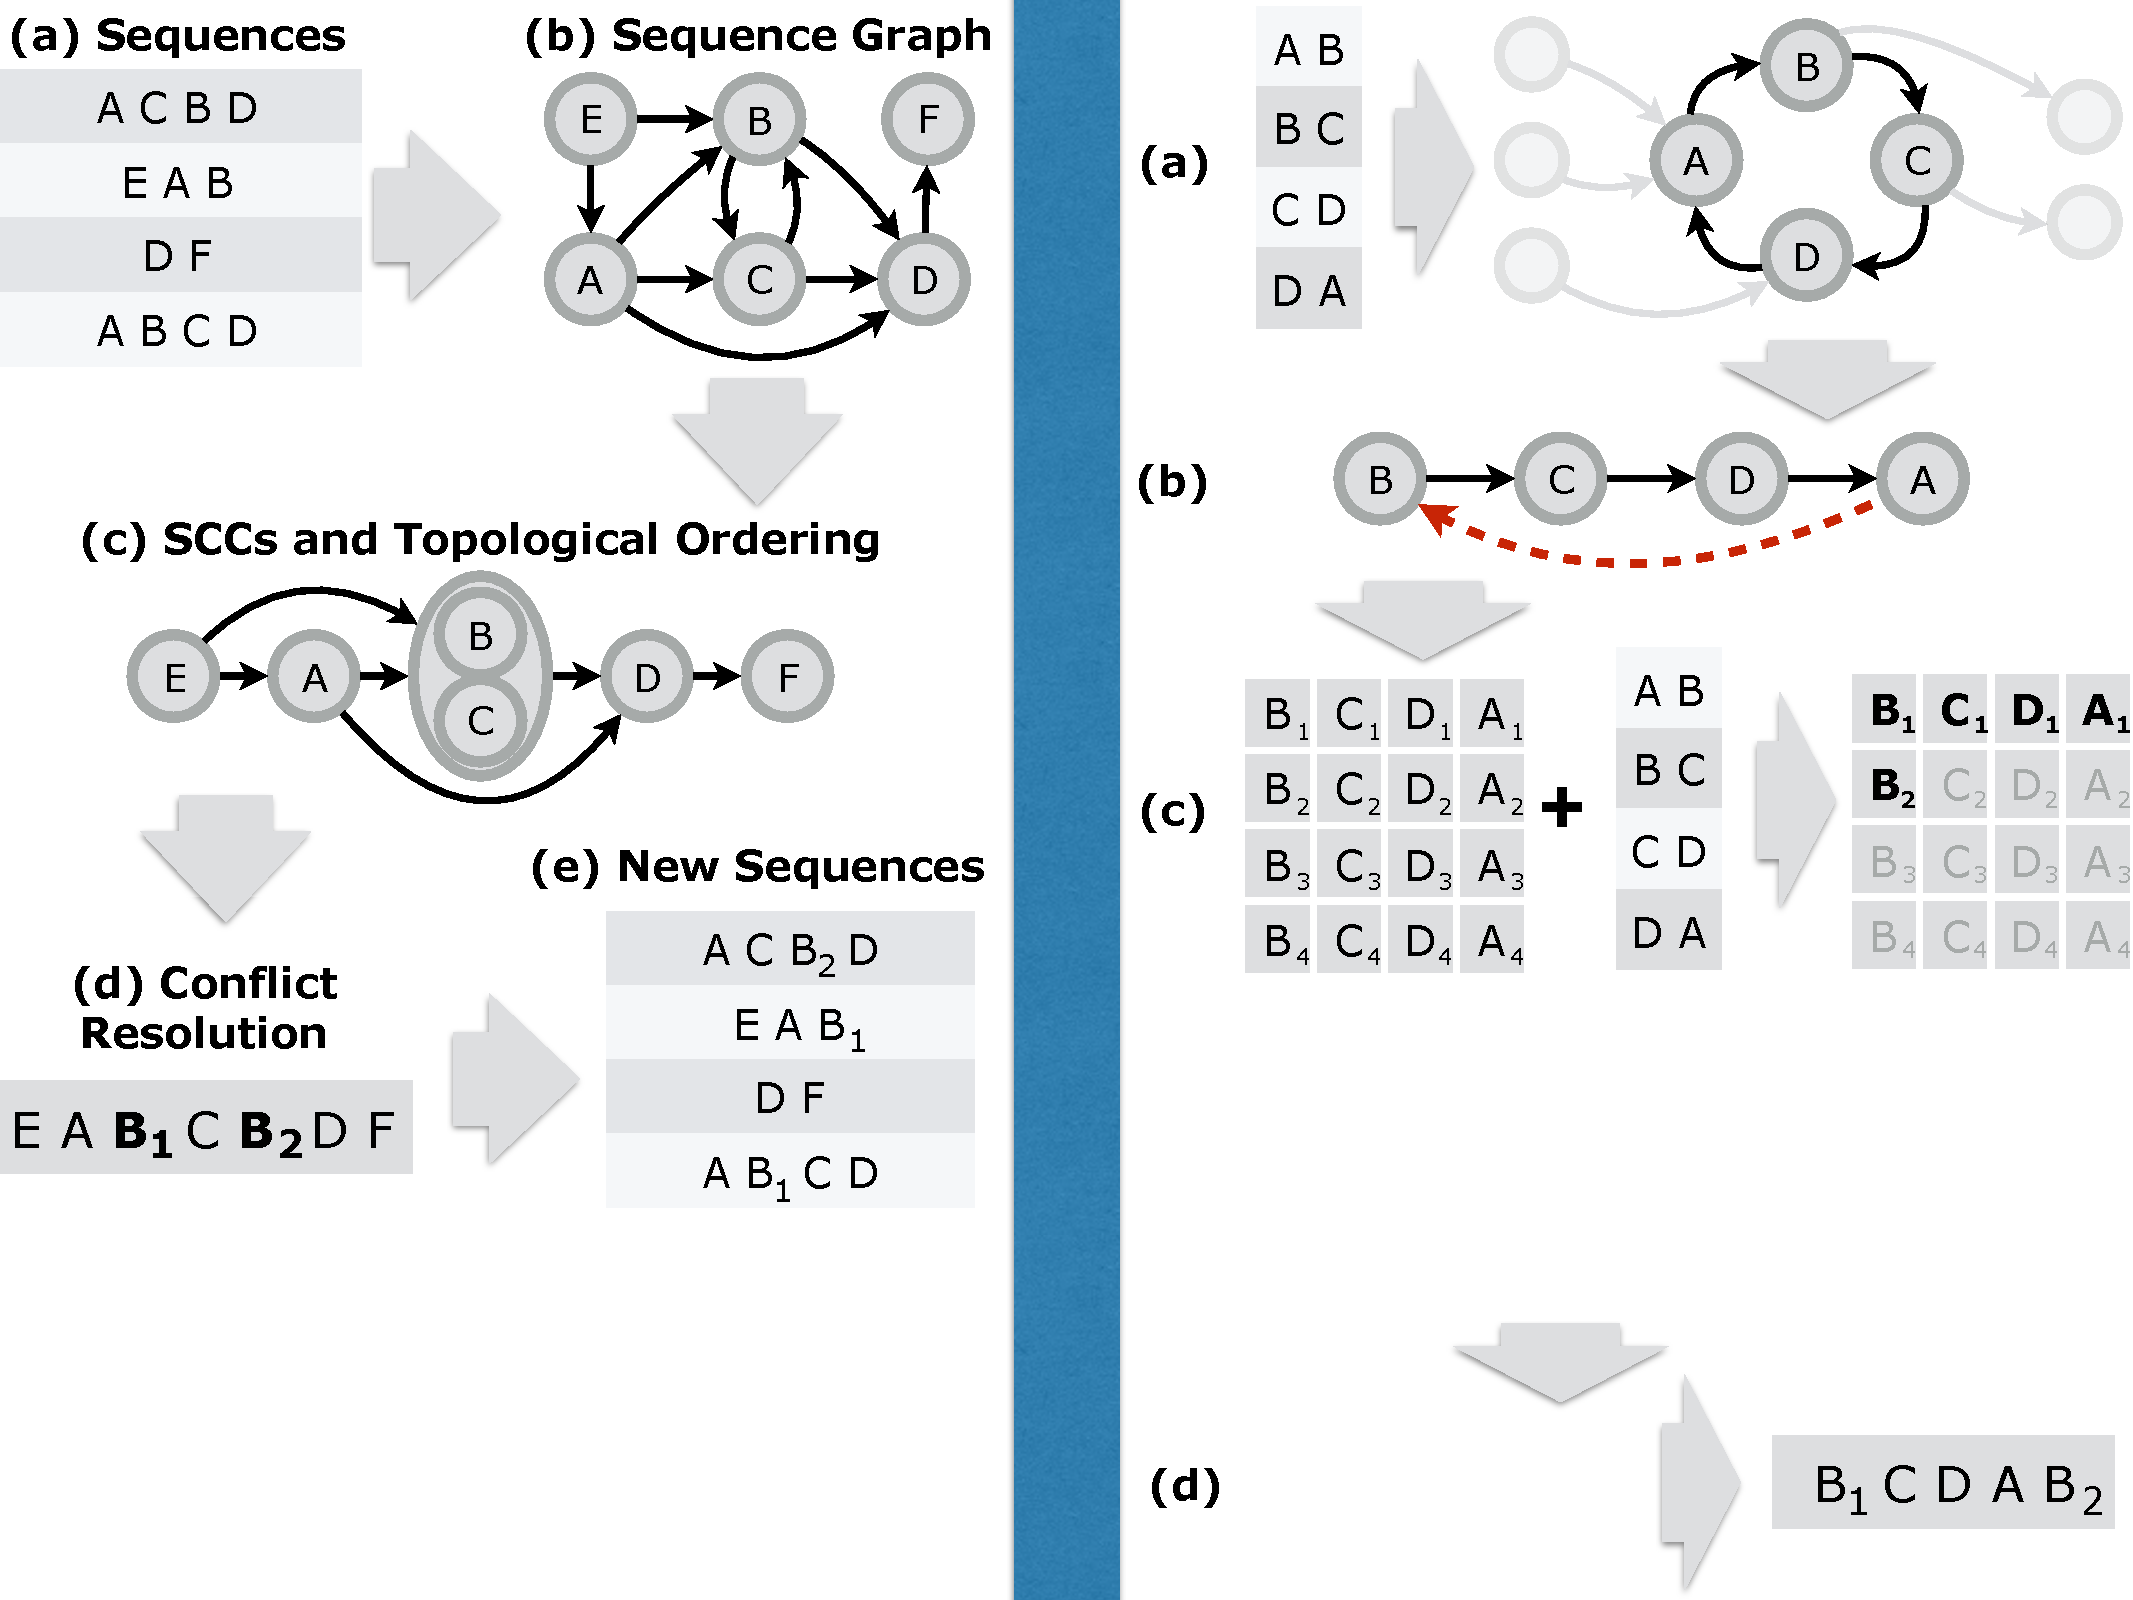
\includegraphics[trim={0 6cm 19.2cm 0}, clip, width=\linewidth]{figures/partial_ordering}
\end{subfigure} 
\end{minipage} 
\caption{This figure shows, at a high level, the process for converting a partial ordering to a total ordering by identifying incomparable elements and creating duplicates to resolve the incomparabilities. (a) shows the four input ordered sequences. In (b), we create a graph of the elements, where there is an edge from $u$ to $v$ if $u$ appears before $v$ in some sequence. (b) shows how the graph can be broken up into an ordered Directed Acyclic Graph (DAG) of Strongly Connected Components (SCC), where each SCC corresponds to a set of incomparable elements. (d) shows the result of splitting elements to resolve incomparability, which is covered in more depth in figure \ref{fig:conflict_res}. In (e), the original sequences are modified with the splits such that each sequence adheres to a total ordering.}
\label{fig:ordering}
\end{figure}



\begin{figure}[t!] 
\begin{minipage}{1\linewidth}
\begin{subfigure}[c]{0.96\linewidth}
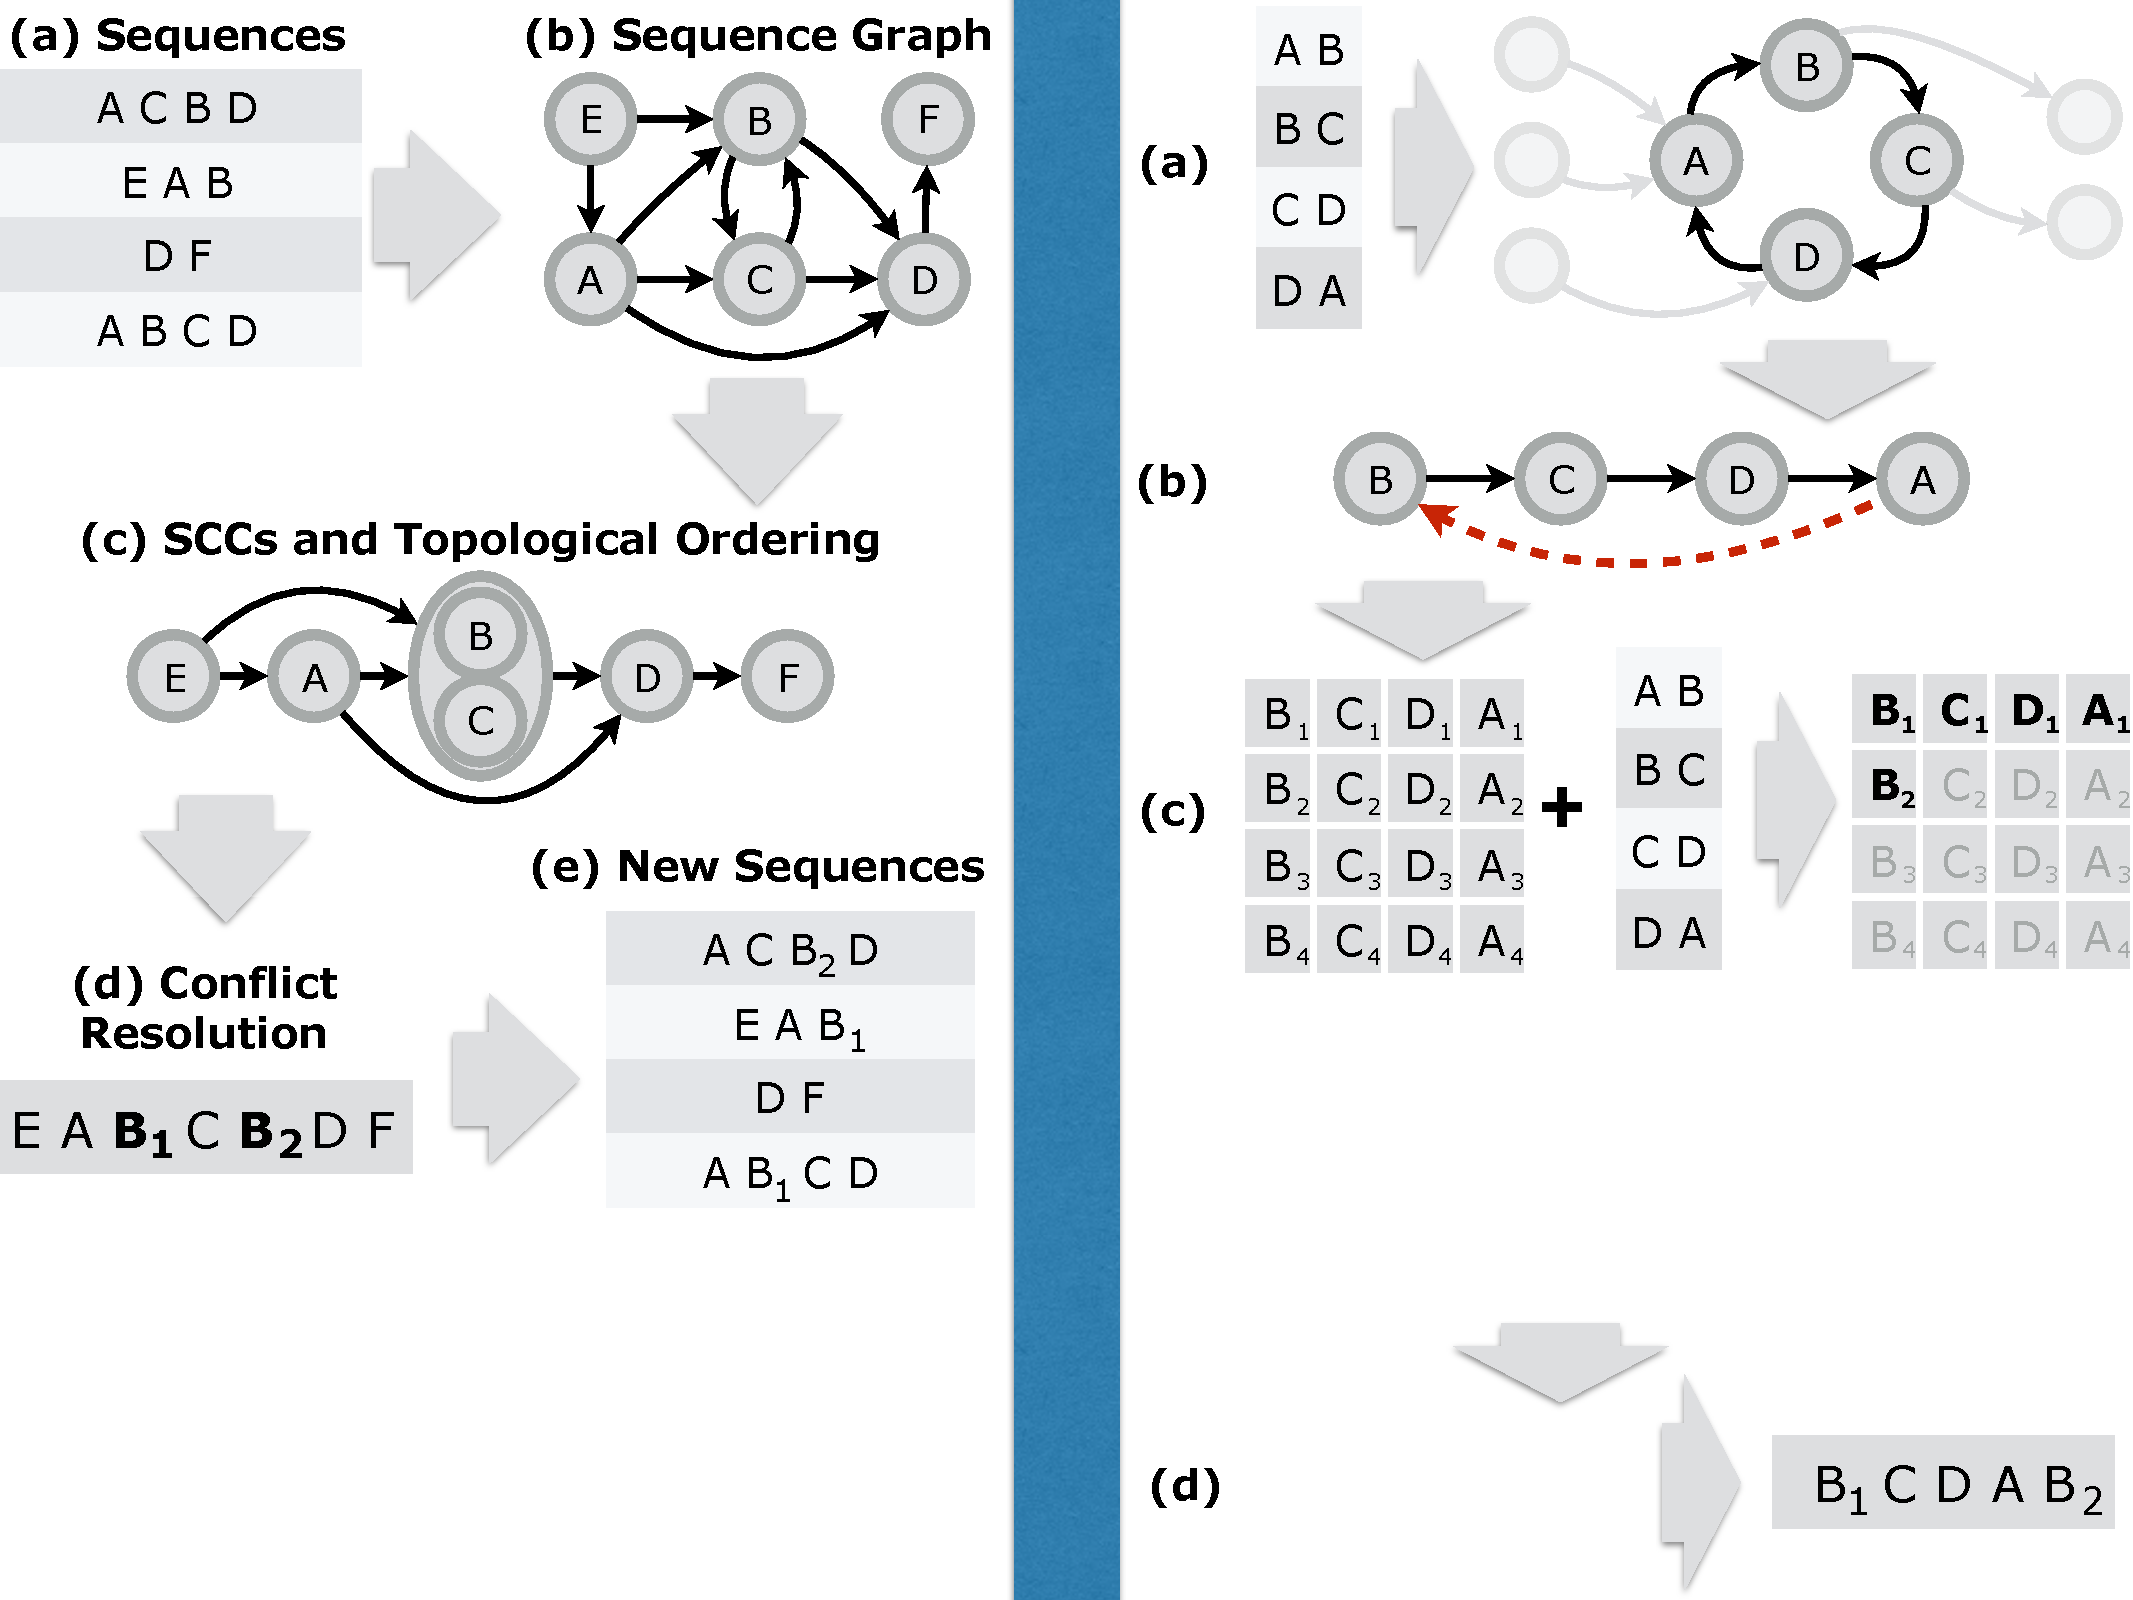
\includegraphics[trim={19.2cm 10cm 0 0}, clip, width=\linewidth]{figures/partial_ordering}
\end{subfigure} 
\end{minipage} 
\caption{This details the Conflict Resolution step of the algorithm. (a) shows a SCC corresponding to four incomparable elements. (b) shows an 'almost' ordering of the SCC nodes, which minimizes the number of backward edges. (c) shows how the almost ordering is used to construct a worst-case quadratically-sized universe, which is then traversed by every sequence to determine which splits are necessary. }
\label{fig:conflict_res}
\end{figure}
\section{Evaluation} \label{sec:evaluation}
SECTION NOT YET UPDATED. Not worth proofreading yet. 

We will now demonstrate the scalability of the supersets encoding scheme table size for a real exchange point. 

\subsection{Experimental Setup}
We used a data set from the AMS-IX exchange point~\cite{ams-ix}, which gave us access to 63 participants advertising over 600,000 prefixes. Although not on the scale of complete data sets of the largest exchange points, the data set is large enough that the partial masks optimization is required to fit masks into the MAC field. Our experiments were run on a laptop with a 4-core CPU running at 2.4GHz and 16GB of RAM.

The exchange point considered does not yet have support for SDN forwarding rules, so instead we simulate the number of forwarding entries required by the outbound policy of a hypothetical participant which is able to see all available route announcements. The participant was given 1000 uniformly random forwarding entries to a uniformly random subset of participants, with each subset size corresponding to a different experiment. 

\subsection{Performance}
We run our evaluations against a RIB dump of AMS-IX retrieved on May 1st, 2016 from the RIPE Routing Information Service raw data webpage~\cite{ris}.

\begin{figure}[t!] 
\begin{minipage}{1\linewidth}
\begin{subfigure}[b]{0.96\linewidth}
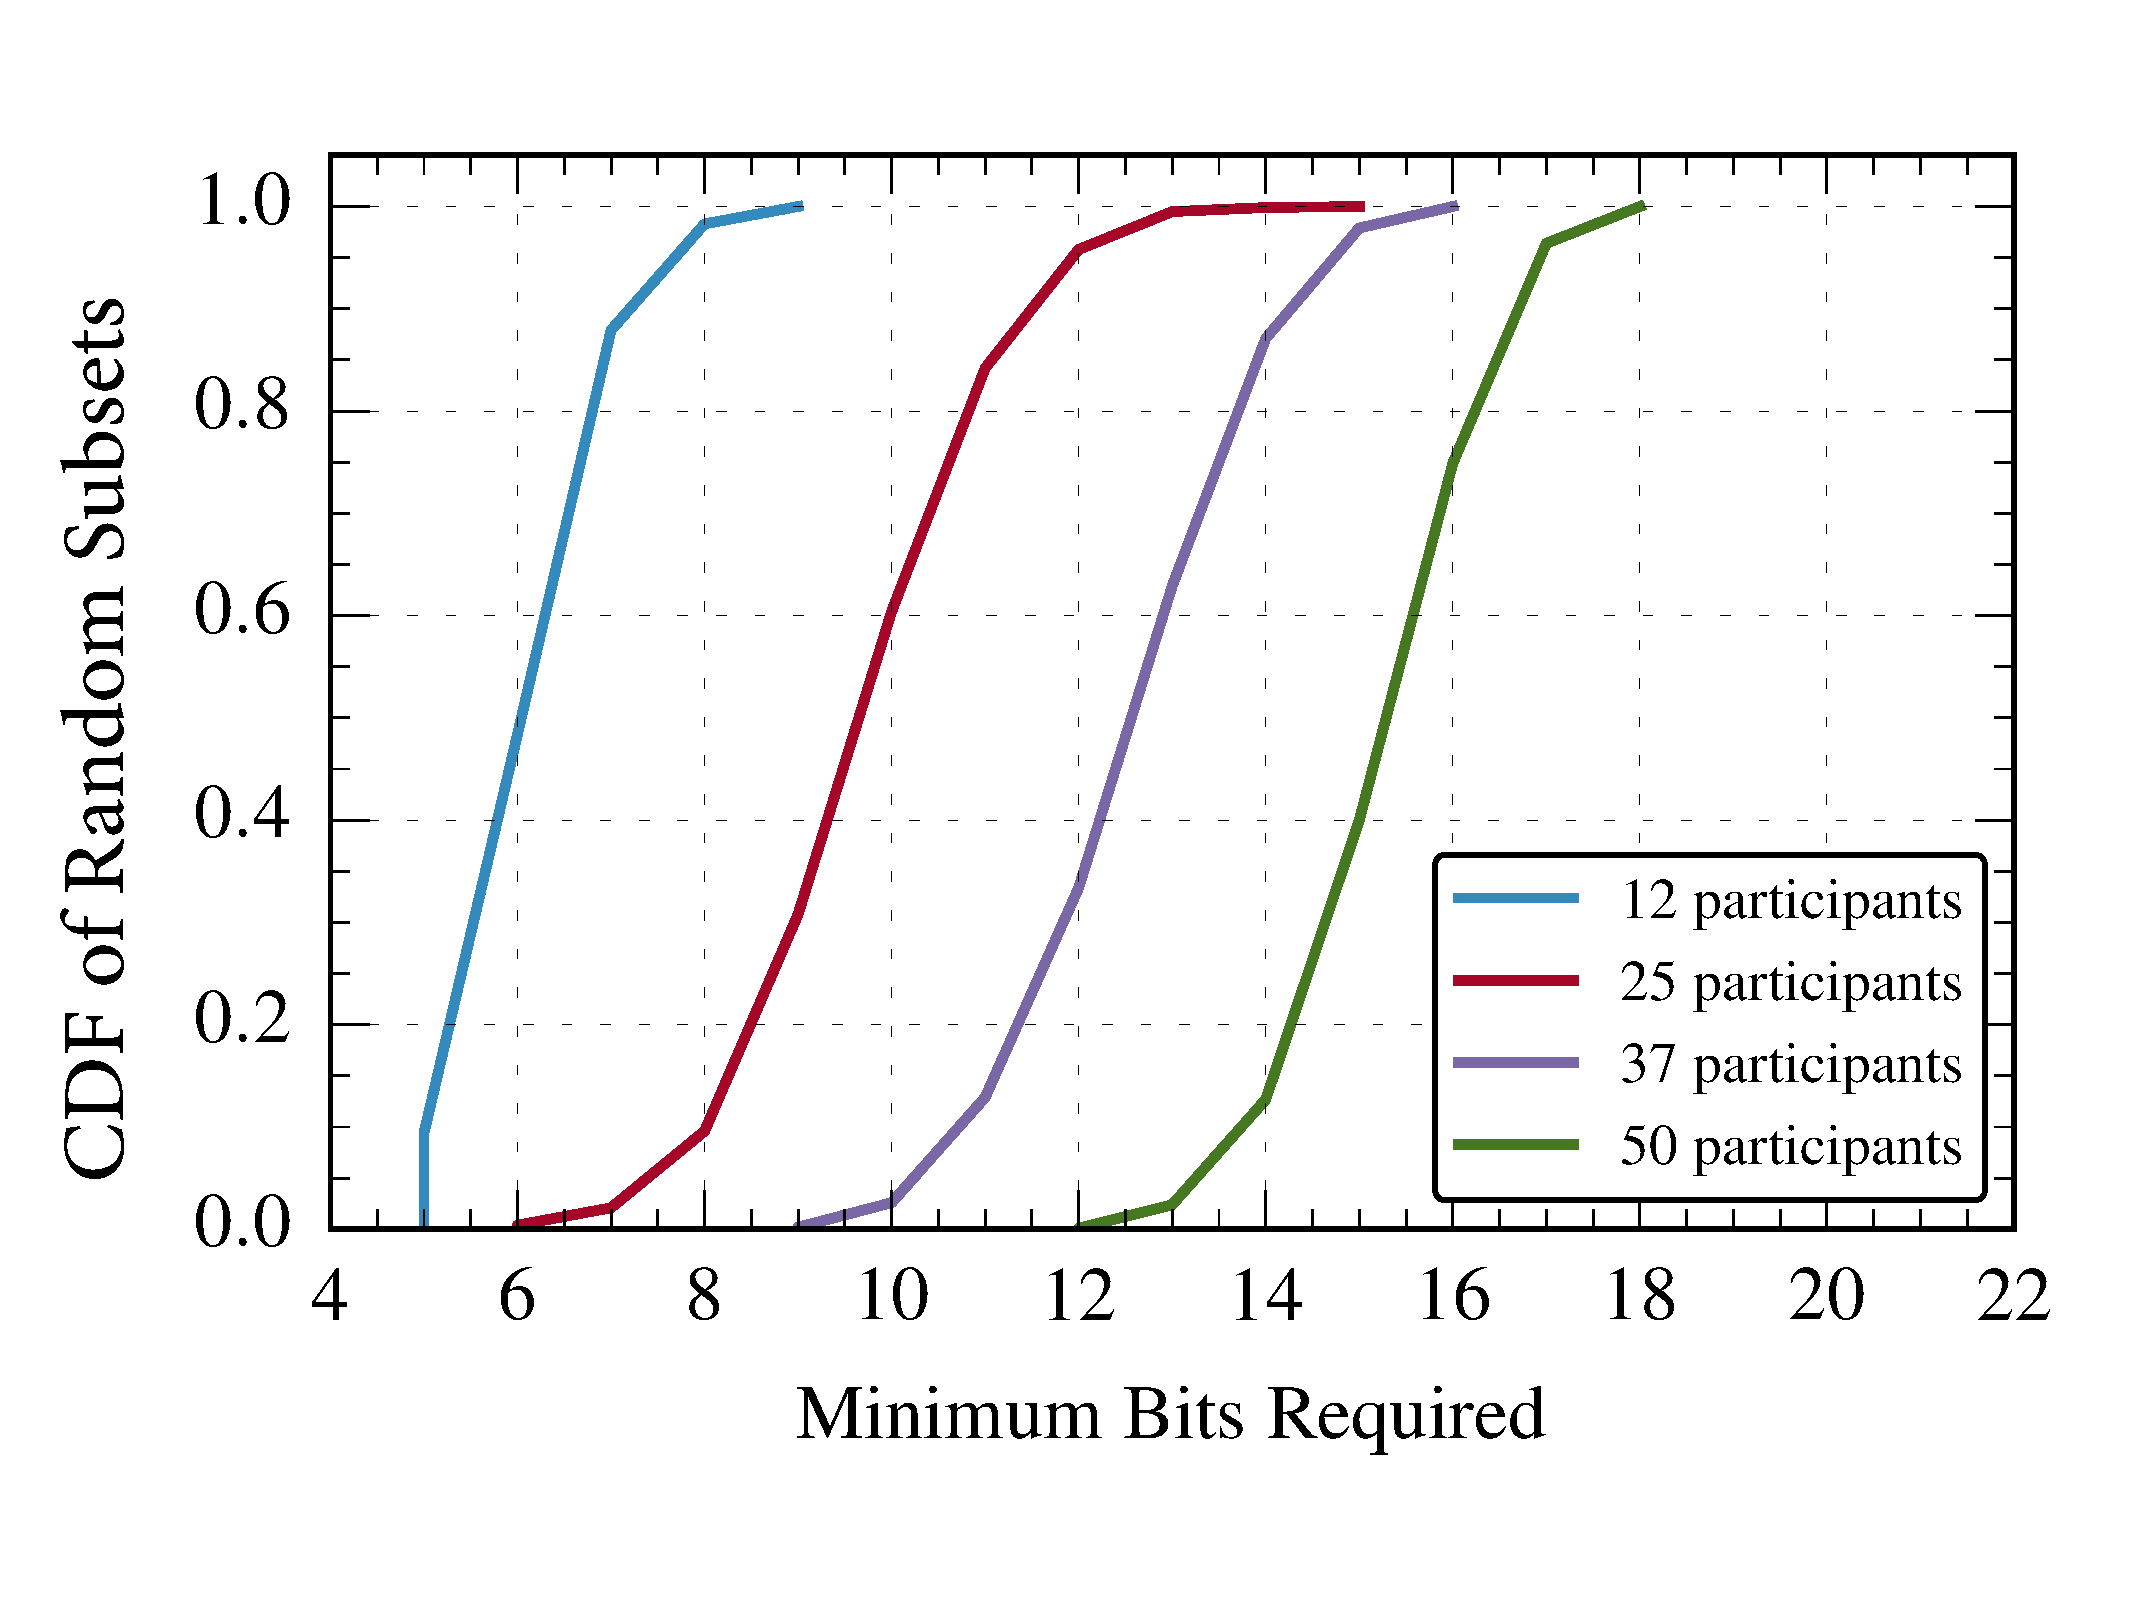
\includegraphics[width=\linewidth]{figures/bit_counts}
\end{subfigure} 
\end{minipage} 
\caption{Minimum number of bits required by a feasible solution for a random policy which forwards to a random subset of participants.}
\label{fig:bits}
\end{figure}

In order for our encoding scheme to successfully work, it must compress the information to the point that it fits into the MAC address field, which is restricted to 48 bits if no other information is encoded alongside reachability. Figure \ref{fig:bits} shows the number of bits required by our reachability encoding with uniformly randomly chosen active sets, repeated 500 times for each active set size. In the worst case, 18 bits were required when considering all 63 participants. The graphs appear to show that the number of bits required scales linearly with the number of participants present in the active set. However, we believe that the number of bits required actually scales sublinearly with the size of the active set, and that the appearance of linear scaling is a consequence of our simulation method. In order for the bits required to scale linearly, the number of participants that simultaneously advertise a single precept would have to also increase linearly in the size of the IXP, but we suspect this is not the case. Even if the number of bits required were indeed to scale linearly, extrapolating out the graph yields that, in the worst case, a participant's active set could contain over 100 participants, allowing very complex forwarding policies.

\begin{figure}[t!] 
\begin{minipage}{1\linewidth}
\begin{subfigure}[b]{0.96\linewidth}
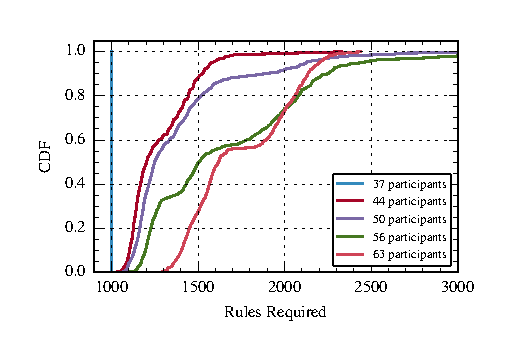
\includegraphics[width=\linewidth]{figures/rule_cdf}
\end{subfigure} 
\end{minipage} 
\caption{Number of rules required after encoding for a random policy of 1000 rules to random subsets of participants.}
\label{fig:rules}
\end{figure}

Figure \ref{fig:rules} shows the number of rules required by our encoding scheme after running the greedy algorithm with a bit limit of 37, allowing 11 bits for the ``mini-MAC". In this experiment, we began with a baseline policy of 1000 rules, with each rule forwarding to a participant chosen uniformly at random from a random active set. The experiment was repeated 500 times for each active set size, and the number of rules required after applying our encoding was plotted. When the active set is of size 37 or fewer, all participants can fit into a single mask, resulting in zero rule inflation. For active sets of size greater than 37, we can see that the inflation factor is at most 2 in the average case and 3 in the worst case for all active sets. 


\begin{figure}[t!] 
\begin{minipage}{1\linewidth}
\begin{subfigure}[b]{0.96\linewidth}
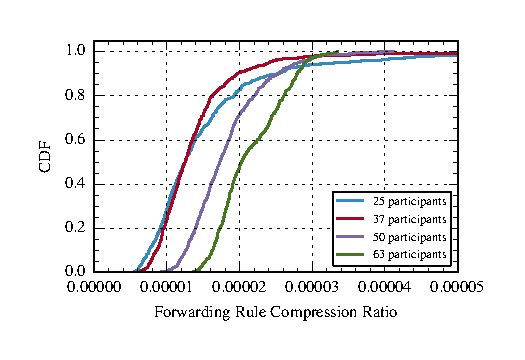
\includegraphics[width=\linewidth]{figures/compression_cdf}
\end{subfigure} 
\end{minipage} 
\caption{Ratio of flow rules required by our encoding algorithm versus the uncompressed
case on random policies involving random subsets of participants.}
\label{fig:compression}
\end{figure}

Figure \ref{fig:compression} shows how the number of flow rules generated by our approach compares to the naive case of zero compression. The compression ratio of our approach versus the naive approach is 20,000 to 1 in the worst case for all active set sizes, and 50,000 to 1 in the median case.


\begin{figure}[t!] 
\begin{minipage}{1\linewidth}
\begin{subfigure}[b]{0.96\linewidth}
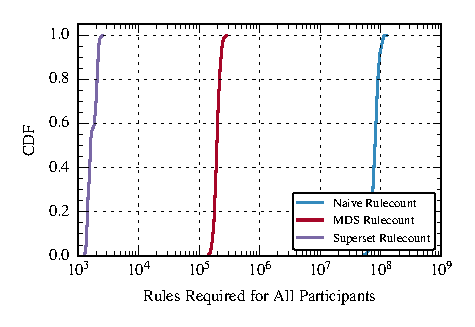
\includegraphics[width=\linewidth]{figures/comparison_cdf}
\end{subfigure} 
\end{minipage} 
\caption{Comparison of the number of flow rules required by our encoding algorithm to the previous state-of-the-art MDS encoding algorithm and the uncompressed case for a random policy involving all participants.}
\label{fig:comparison}
\end{figure}


Figure \ref{fig:comparison} compares our approach to the uncompressed case, as well as to the previous state-of-the-art, the MDS algorithm used in the original SDX system~\cite{gupta2014sdx}. The comparisons were made using the same approach of generating 1000 random rules, except for the MDS simulation. The MDS algorithm requires each prefix's default next-hop as part of the input, so in each trial we chose next-hops uniformly at random from the list of available next-hops. The graph shows that our approach consistently compresses the number of flow rules by two orders of mangitude greater than the MDS algorithm, which itself compressed the number of flow rules required by the naive case by three orders of magnitude. 

\begin{figure}[t!] 
\begin{minipage}{1\linewidth}
\begin{subfigure}[b]{\linewidth}
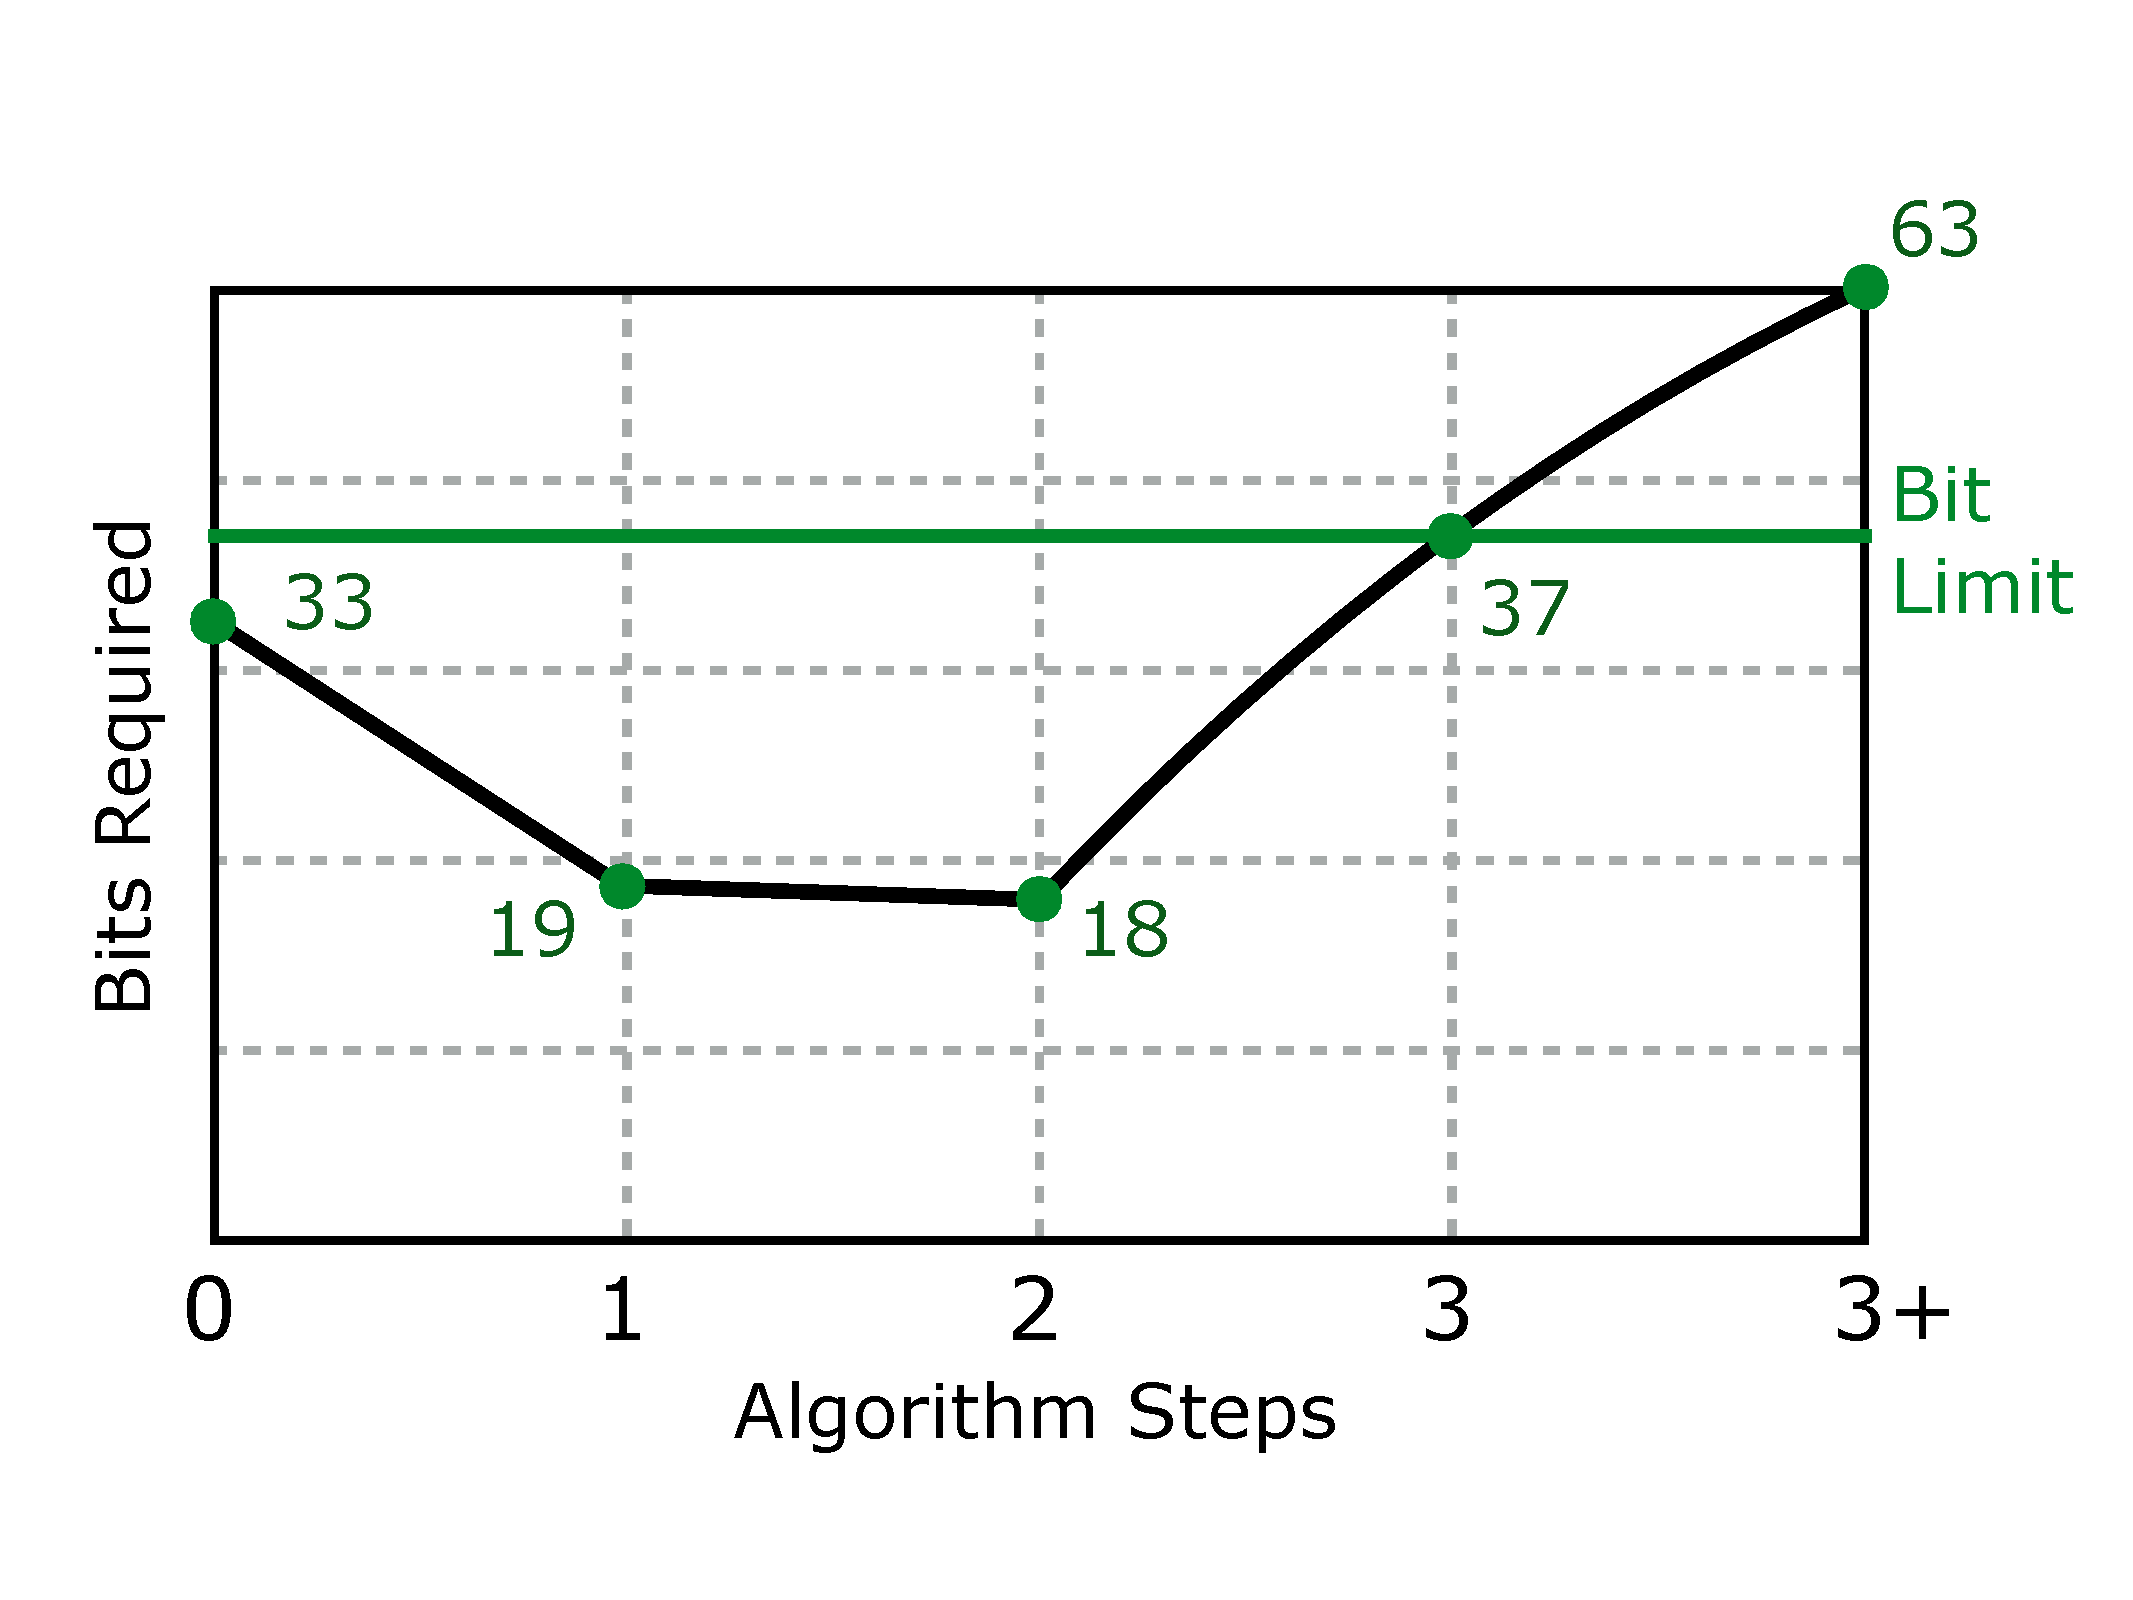
\includegraphics[width=\linewidth]{figures/bit_graph}
\end{subfigure} 
\end{minipage} 
\caption{Graph of the number of bits required by the encoding scheme at each step of the algorithm, shown with real values computed over the AMS-IX RIPE data set. Step 0 is the input of all sets, step 1 is removal of subsets, step 2 is attempting greedy bit minimization, step 3 is after greedily decreasing inflation up to the bit limit, and step 3+ is with no bit limit. }
\label{fig:bit_graph}
\end{figure}
\section{Related Work} \label{sec:related}

Variable-length prefix codes have been used for various applications. In the seminal work of Huffman~\cite{Huffman} an algorithm for an optimal selection of them was described for lossless compression of a source symbol. The selection minimizes the encoding length by using fewer bits for common symbols, achieving results close to lower bounds from information theory. More recently, they were suggested to encode paths as a sequence of nodes while focusing one reducing the maximum length of any encoded path~\cite{PathEncoding}. A similar approach was suggested for the encoding for fixed-width memories~\cite{FixedMemories}. In all these schemes, the encoding is given by the concatenating the codes of the attributes, thus is often long for a large number of possible attributes. On the contrary, in the suggested scheme the dependency is only in the number of unique groups and the number of attributes in a set.


Alpaca~\cite{alpaca} also aims to embed attributes of each flow into the packet header with the goal of easing network policy enforcement, but does not follow the FEC tagging abstraction. Instead, they embed attributes into the hosts' IP address assignments, which adds the constraint that attribute encodings must be unique for each host. 

Flowtags~\cite{flowtags} uses flat tagging to associate each packet with a source host and a middlebox path, even in the face of middleboxes which modify packet headers. Their approach relies upon modifications of the source code of each middlebox to be able to read and write the tags. Our approach allows middleboxes to be unaware of tags, but at the cost of having no source host association which is readable by middleboxes. Tags are attached to packets by the first middlebox that the packets traverse. This implies that the packets must be steered to the first middlebox by some other means. Rules for decoding the tags are installed reactively as network nodes see tags for the first time. 

The SDX~\cite{sdx} project uses flat tagging to attach to packets a list of valid next-hops that packets can take through an internet exchange point . This list is then used to correctly enforce interdomain SDN policies that exchange point members install themselves. Tags are attached to packets by controller responses to ARP requests with tags as the destination MAC addresses. Rules for decoding the tags are installed proactively in the exchange point fabric.

SDX was followed by the iSDX~\cite{isdx} project, which aimed to address some of the scalability challenges that the first project faced. Namely, the number of rules needed to decode tags was prohibitively large in SDX, preventing any reasonably-sized IXP from implementing the project on commodity switches. One of the key changes that the iSDX project made to improve scalability was the introduction of a new tagging scheme which utilized wildcard matching. This tagging scheme is the precursor to our work. The tag attachment and decoding model mimicked the first SDX.

Bloom filter~\cite{Bloom} is a popular data structure for set representation. It supports membership queries and relies on a bit array. Bloom filter suffers from an inherent false positive error, where some elements can be wrongly reported as members of the set. While minimizing the tag width is an key property of our scheme, the Bloom filter memory is several times larger than the number of elements, e.g. 10-20 times for a false positive probability of 0.01\% - 1\%. Moreover, Bloom filter relies on hashing which might not be available in some switch architectures.


\input{Conclusion}

%\end{sloppypar}

%\vspace{-0.01in}
%\section*{Acknowledgments}
% Comments for people we need to acknowledge in the final version.
\noindent \textbf{Acknowledgments.}
Fill me in
%\pagebreak
%\small
%\setlength{\bibsep}{0pt}
%\setlength{\parskip}{-1pt}
%\setlength{\itemsep}{-1pt}
% \footnotesize % SPACE
\balance
\bibliography{paper}
\bibliographystyle{acm}
%\bibliographystyle{abbrvnat_noaddr} % SPACE
%\theendnotes % ENDNOTES
}{% onlyAbstract
}

%\pagebreak
%\input{appendix}

\end{document}

%%%%%%%%%%%%%%%%%%%%  END OF DOCUMENT  %%%%%%%%%%%%%%%%%%%%
